\chapter{Results: \deploy Demonstration}
In this chapter, \deploy's capabilities is demonstrated 
for a simple and complex case.  
This chapter will be broken into two sections: 
\begin{enumerate}
    \item \deploy demonstration for simple transition scenarios
    \item \deploy demonstration for the EG01-30 transition scenario
\end{enumerate}

\section{\deploy Demonstration of Simple Transition Scenarios}
\label{sec:demo}

This section demonstrates \deploy's capability 
to effectively set up a simple transition scenario simulation 
for constant, linearly increasing, and 
sinusoidal power demand simulations.
These simulations only include
three facility types: \texttt{source}, \texttt{reactor}, and 
\texttt{sink}. 
The simulations begin with ten \texttt{reactor} facilities 
(\texttt{reactor1} to \texttt{reactor10}). 
These reactors have staggered cycle lengths and lifetimes to prevent 
simultaneous refueling and setup gradual decommissioning. 
\deploy is configured to deploy \texttt{new reactor} facilities
to meet the loss of power supply created by the decommissioning 
of the initial \texttt{reactor} facilities. 
Table \ref{tab:demonstrations} shows the 
\deploy input parameters for these simulations.
Figure \ref{fig:powerplots} shows the user-defined power demand curves 
for the three simulations that \deploy deploys facilities to meet.

\begin{table}[]
    \resizebox{\textwidth}{!}{%
    \begin{tabular}{l|l|c|l|l}
    \hline
    \multirow{2}{*}{}                         & \multicolumn{1}{c|}{\multirow{2}{*}{\textbf{Input Parameter}}} & \multicolumn{3}{c}{\textbf{Simulation Description}}                                                                                                                                                                                                                                                       \\ \cline{3-5} 
                                              & \multicolumn{1}{c|}{}                                          & \multicolumn{1}{l|}{\textbf{Constant Power}}                                                                 & \textbf{\begin{tabular}[c]{@{}l@{}}Linearly Increasing \\ Power\end{tabular}}                  & \textbf{Sinusoidal Power}                                                                  \\ \hline
    \multirow{5}{*}{\textbf{Required Inputs}} & Demand driving commodity                                       & \multicolumn{3}{c}{Power}                                                                                                                                                                                                                                                                                 \\ \cline{2-5} 
                                              & Demand equation                                                & \multicolumn{1}{l|}{10000 MW}                                                                                & \begin{tabular}[c]{@{}l@{}}t\textless 40: 10000 MW\\ t\textgreater{}=40: 250*t MW\end{tabular} & 1000*$\sin(\pi*t/3)$+10000                                                                 \\ \cline{2-5} 
                                              & Facilities it controls                                         & \multicolumn{3}{c}{Source, reactor, sink}                                                                                                                                                                                                                                                                 \\ \cline{2-5} 
                                              & Prediction method                                              & \multicolumn{1}{l|}{\begin{tabular}[c]{@{}l@{}}Power: \texttt{FFT}\\ Fuel: \texttt{MA}\\ Spent fuel: \texttt{MA}\end{tabular}}          & \begin{tabular}[c]{@{}l@{}}Power: FFT\\ Fuel: MA\\ Spent fuel: FFT\end{tabular}                & \begin{tabular}[c]{@{}l@{}}Power: HW\\ Fuel: MA\\ Spent fuel: FFT\end{tabular}             \\ \cline{2-5} 
                                              & Deployment Driving Method                                      & \multicolumn{3}{c}{Installed Capacity}                                                                                                                                                                                                                                                                    \\ \hline
    \multirow{2}{*}{\textbf{Optional Inputs}} & Buffer type                                                    & \multicolumn{3}{c}{Absolute}                                                                                                                                                                                                                                                                              \\ \cline{2-5} 
                                              & Buffer size                                                    & \multicolumn{1}{l|}{\begin{tabular}[c]{@{}l@{}}Power: 3000 MW\\ Fuel: 0 kg \\ Spent fuel: 0 kg\end{tabular}} & \begin{tabular}[c]{@{}l@{}}Power: 2000 MW\\ Fuel: 1000 kg \\ Spent fuel: 0 kg\end{tabular}     & \begin{tabular}[c]{@{}l@{}}Power: 2000 MW\\ Fuel: 1000 kg \\ Spent fuel: 0 kg\end{tabular} \\ \hline
    \end{tabular}%
    }
    \caption{\deploy's input parameters for the basic transition scenarios.}
    \label{tab:demonstrations}
    \end{table}

    \begin{figure}[]
        \begin{center}
            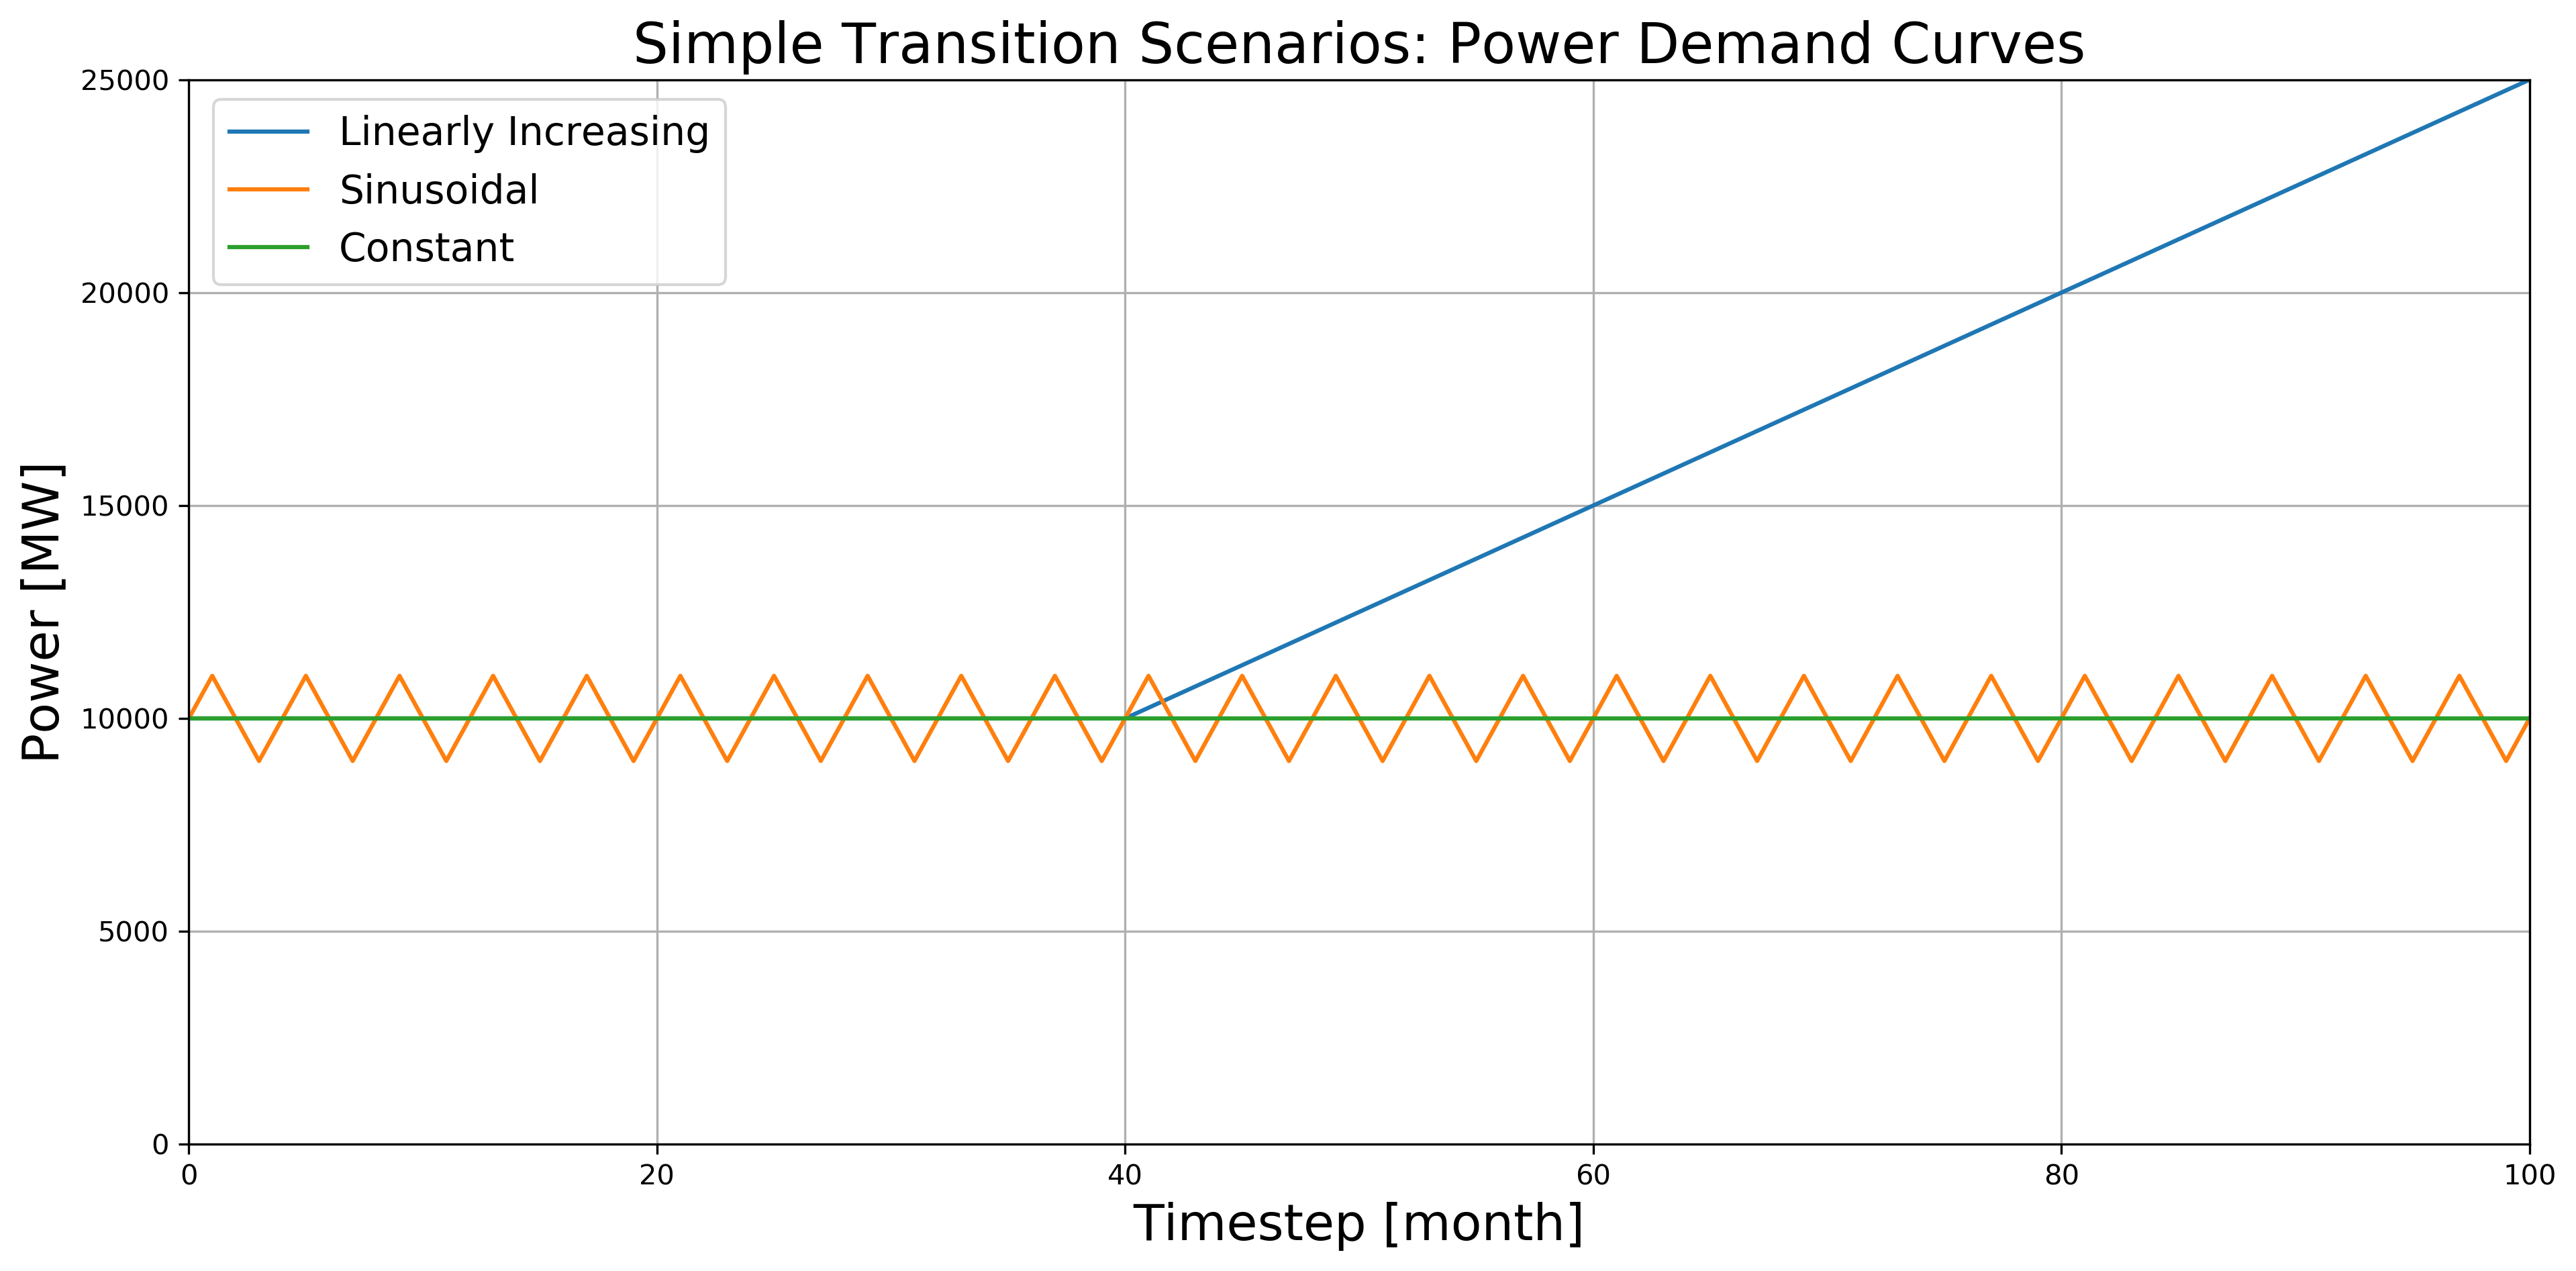
\includegraphics[scale=0.5]{./figures/powerplots.png}
        \end{center}
            \caption{Power demand curves for basic transition scenarios.}
        \label{fig:powerplots}
    \end{figure}

\subsection{Simple Transition Scenario Simulation: Constant Demand}
Figures \ref{fig:constanttransition-power}, \ref{fig:constanttransition-fuel},
and \ref{fig:constanttransition-spentfuel} demonstrate \deploy's capability 
to deploy reactor and supporting facilities to meet the
constant power demand and subsequently demanded 
secondary commodities with minimal undersupply. 
Table \ref{tab:transition-scenario-results} shows the number of 
undersupplied timesteps. 
In Figure \ref{fig:constanttransition-power}, there exist no time steps 
in which the supply of power falls under demand, meeting the main 
objective of \deploy. 
By using a combination of the \texttt{FFT} method for 
predicting demand and setting the power supply buffer to 3000MW 
(the capacity of 3 reactors), the user minimizes the number of 
undersupplied timesteps for every commodity.

In figure \ref{fig:constanttransition-fuel},
a large-throughput source facility is initially
deployed to meet the large initial fuel demand for the commissioning 
of ten reactors. 
By having a large-throughput source facility exist for the 
first few time steps, \deploy does not deploy supporting
facilities that become redundant at later times in  
the simulation.
This reflects reality in which reactor manufacturers accumulate
an appropriate amount of fuel inventory before starting 
up reactors. 
There is one time step in which a power undersupply exists after the 
decommissioning of the large initial facility; 
this is unavoidable as the prediction methods in \deploy are 
unable to foresee this sudden drop in demand. 

    \begin{figure}[]
        \centering
        \begin{subfigure}[t]{\textwidth}
        \centering
            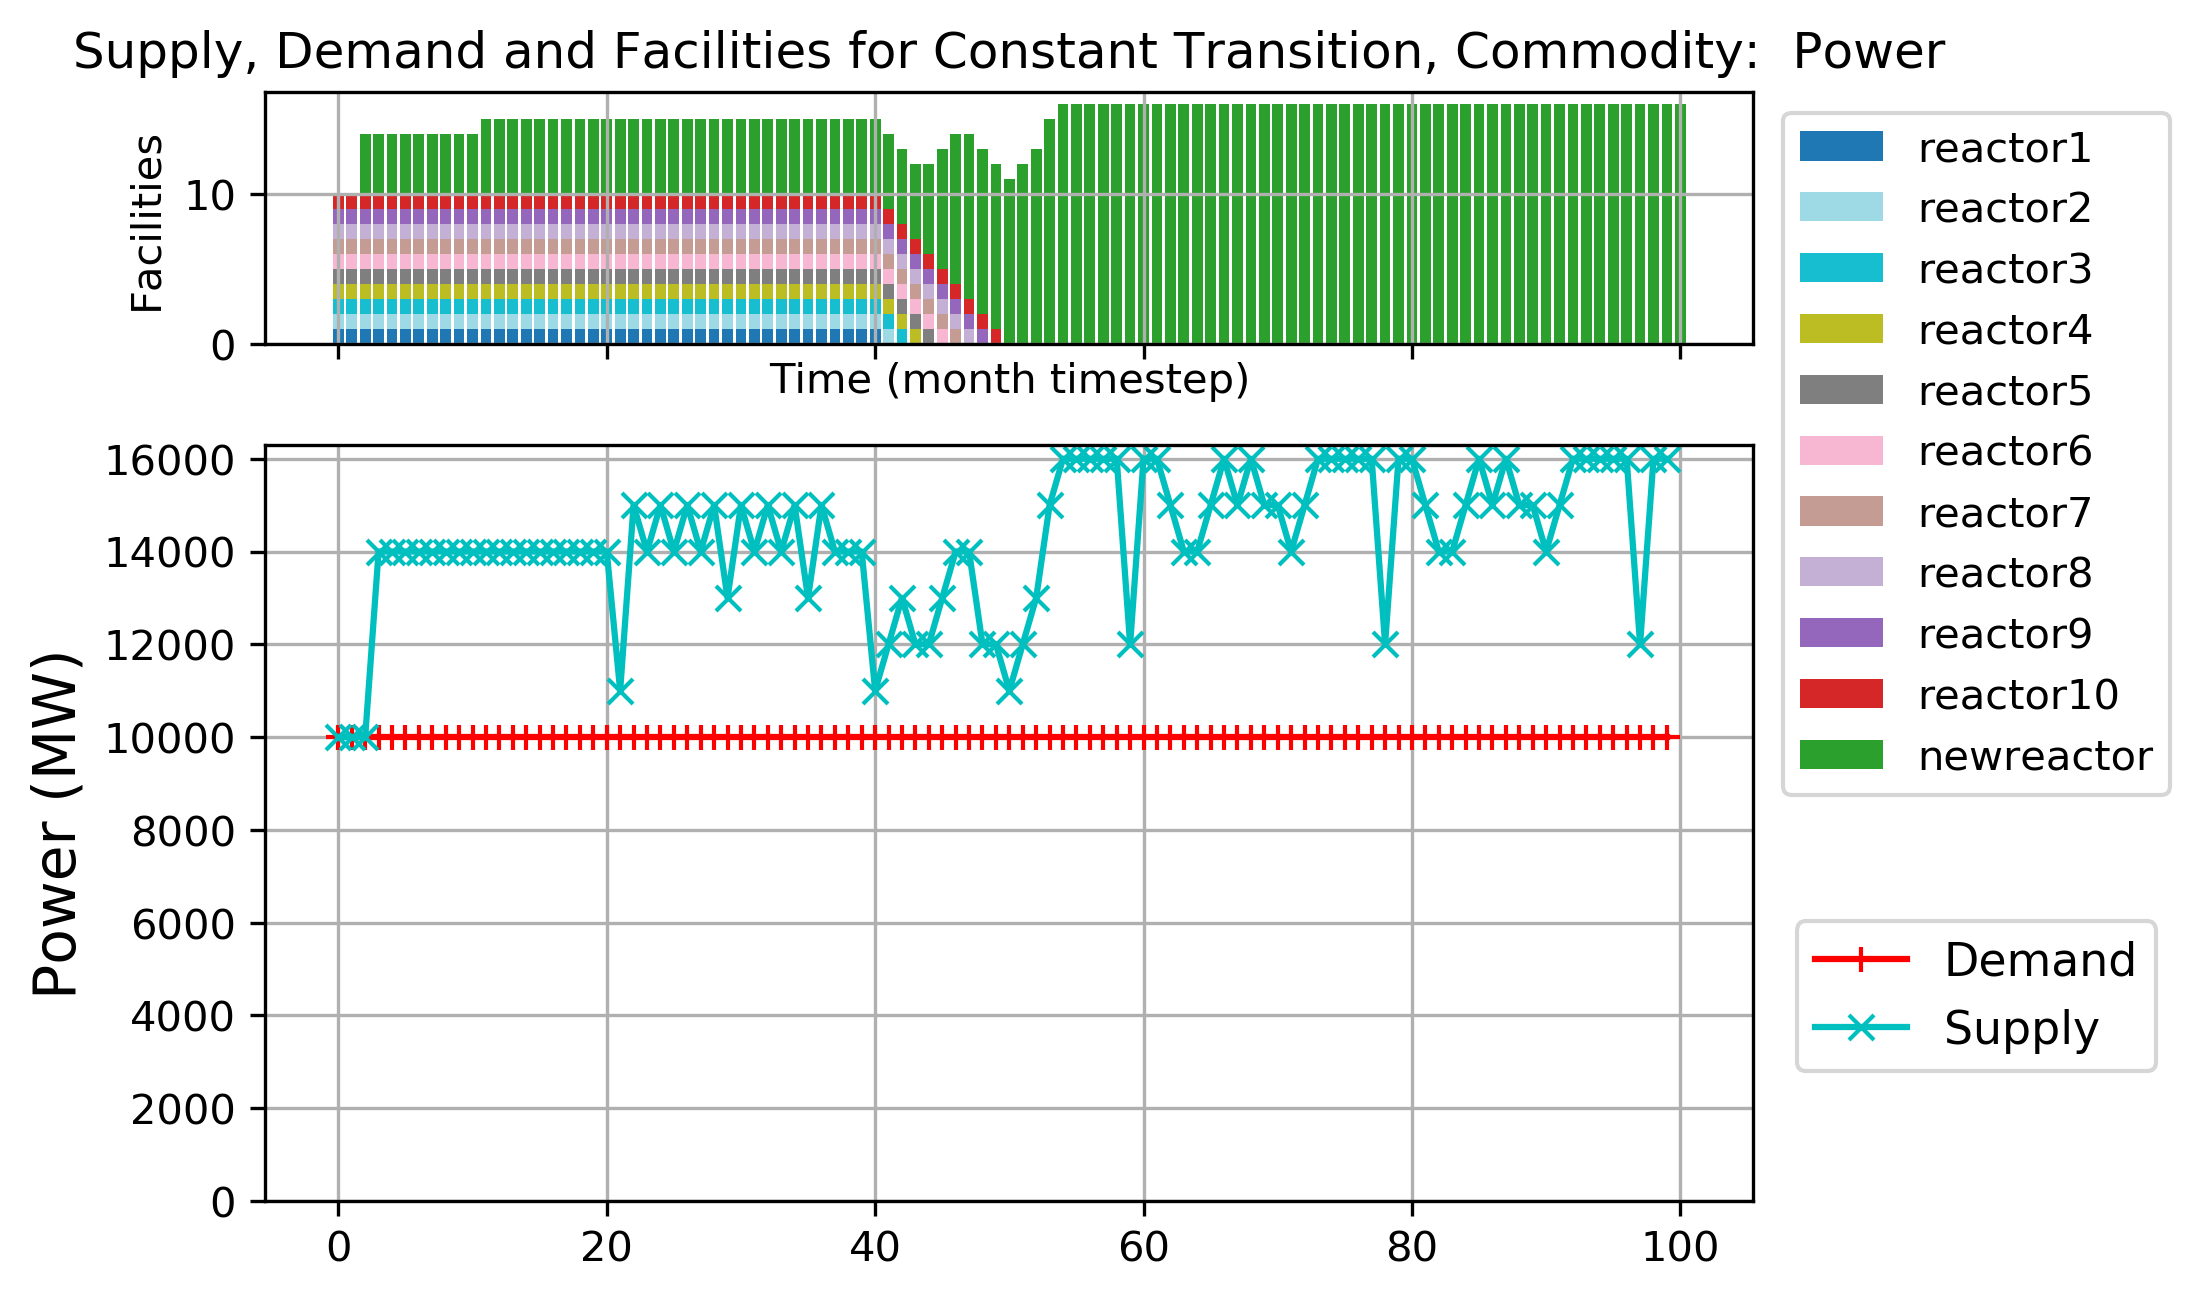
\includegraphics[width=0.7\linewidth]{figures/constanttransition-power.png} 
            \caption{The power demand is a user-defined equation and power is supplied by the reactors.}
            \label{fig:constanttransition-power}
        \end{subfigure}
        \begin{subfigure}[t]{0.6\textwidth}
            \centering
            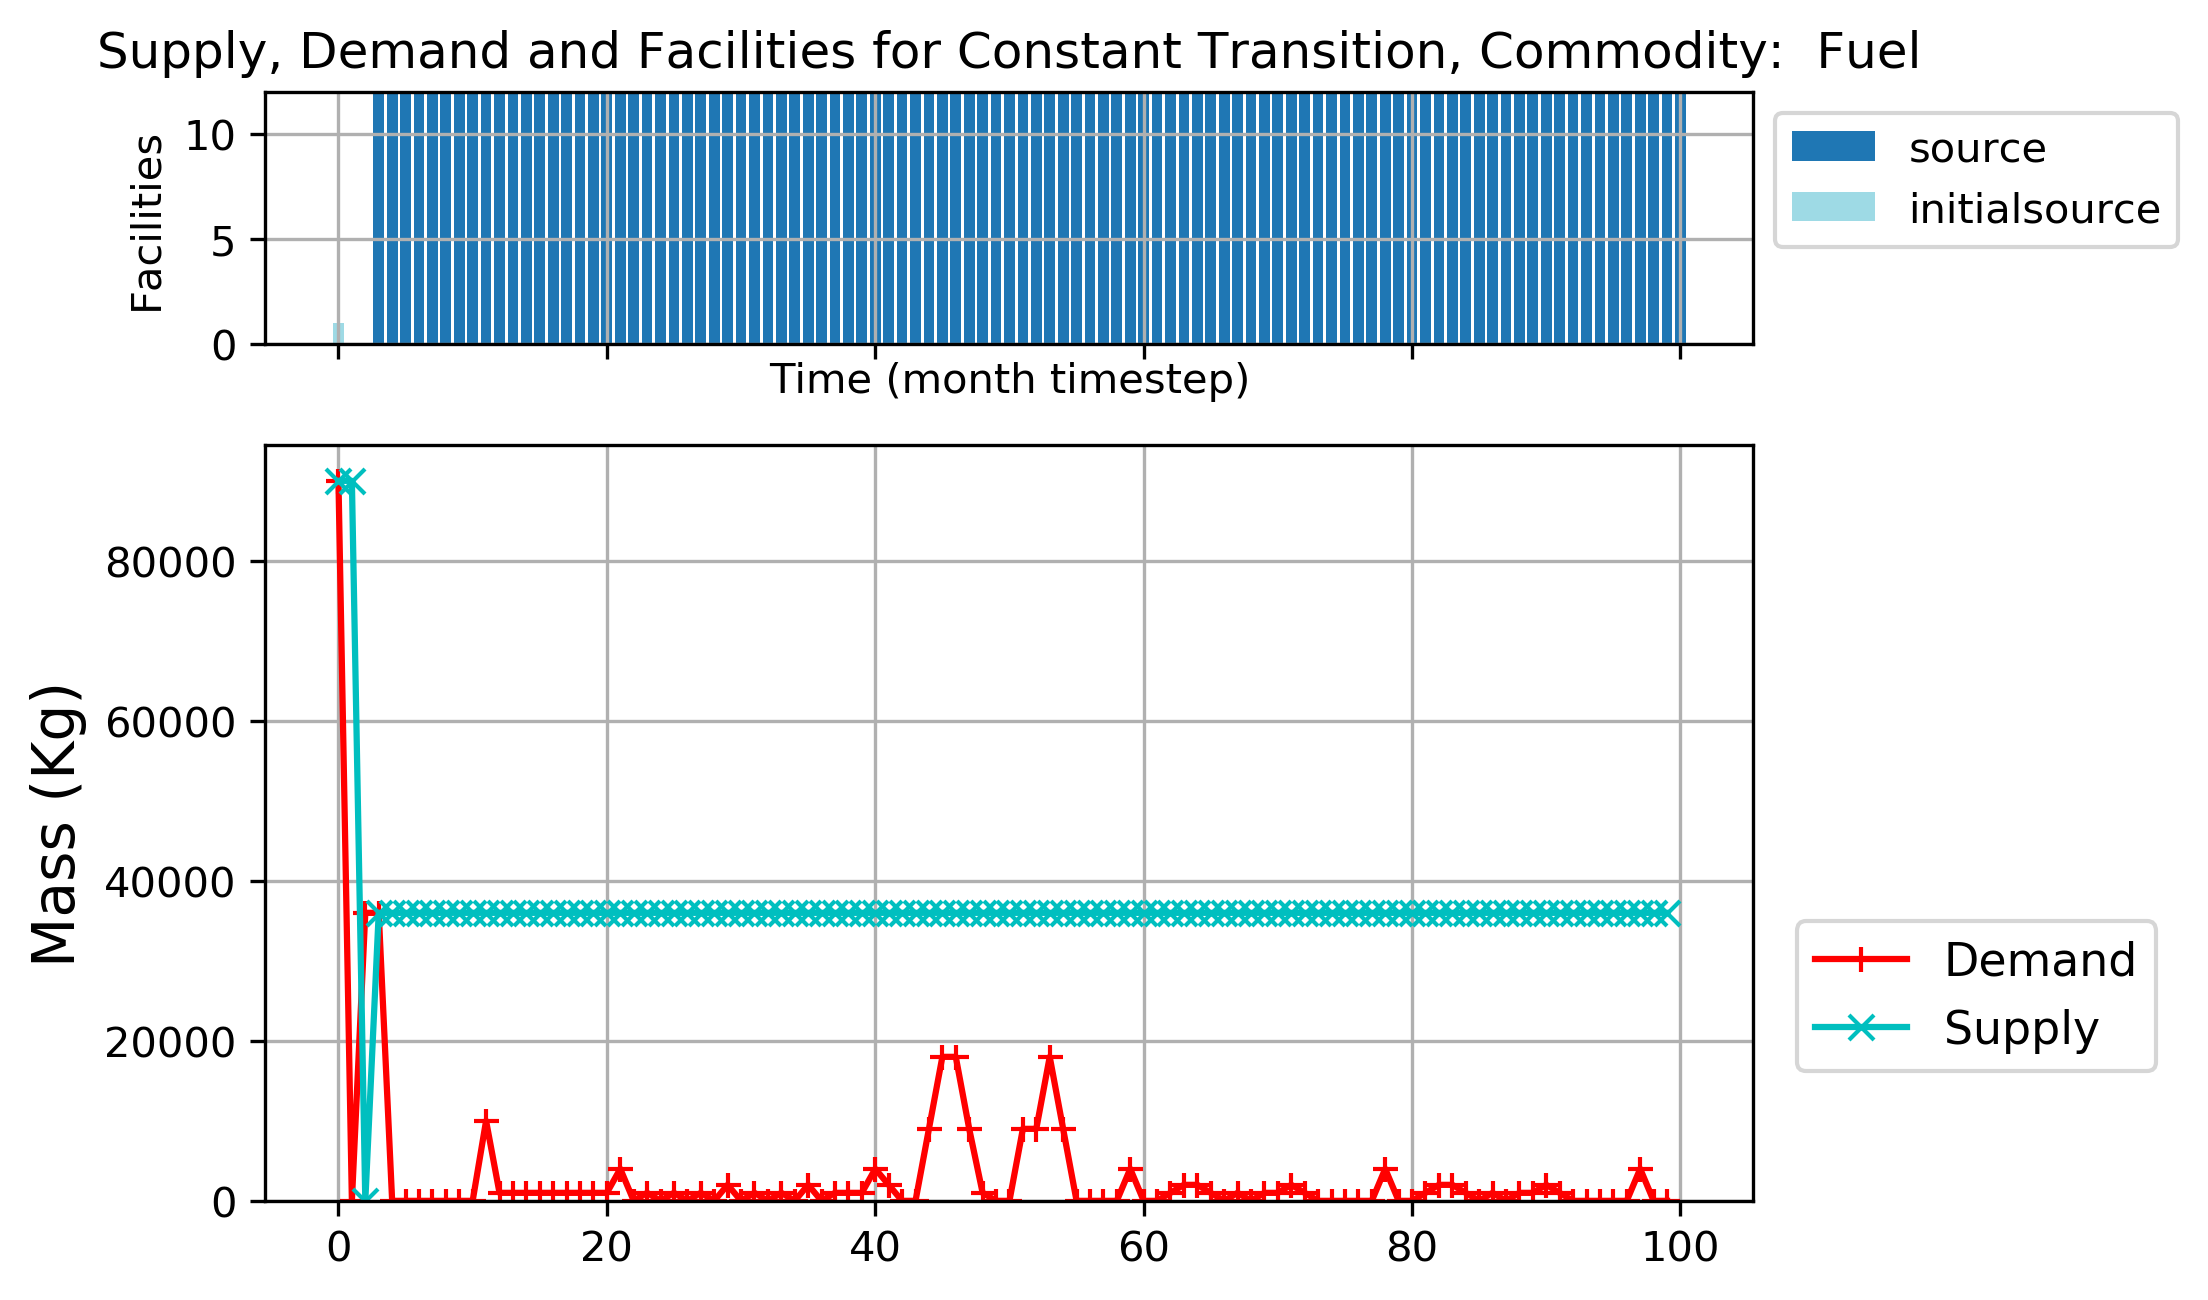
\includegraphics[width=\linewidth]{figures/constanttransition-fuel.png} 
            \caption{Fuel is demanded by reactors and supplied by source facilities.}
            \label{fig:constanttransition-fuel}
        \end{subfigure}
        \begin{subfigure}[t]{0.6\textwidth}
            \centering
            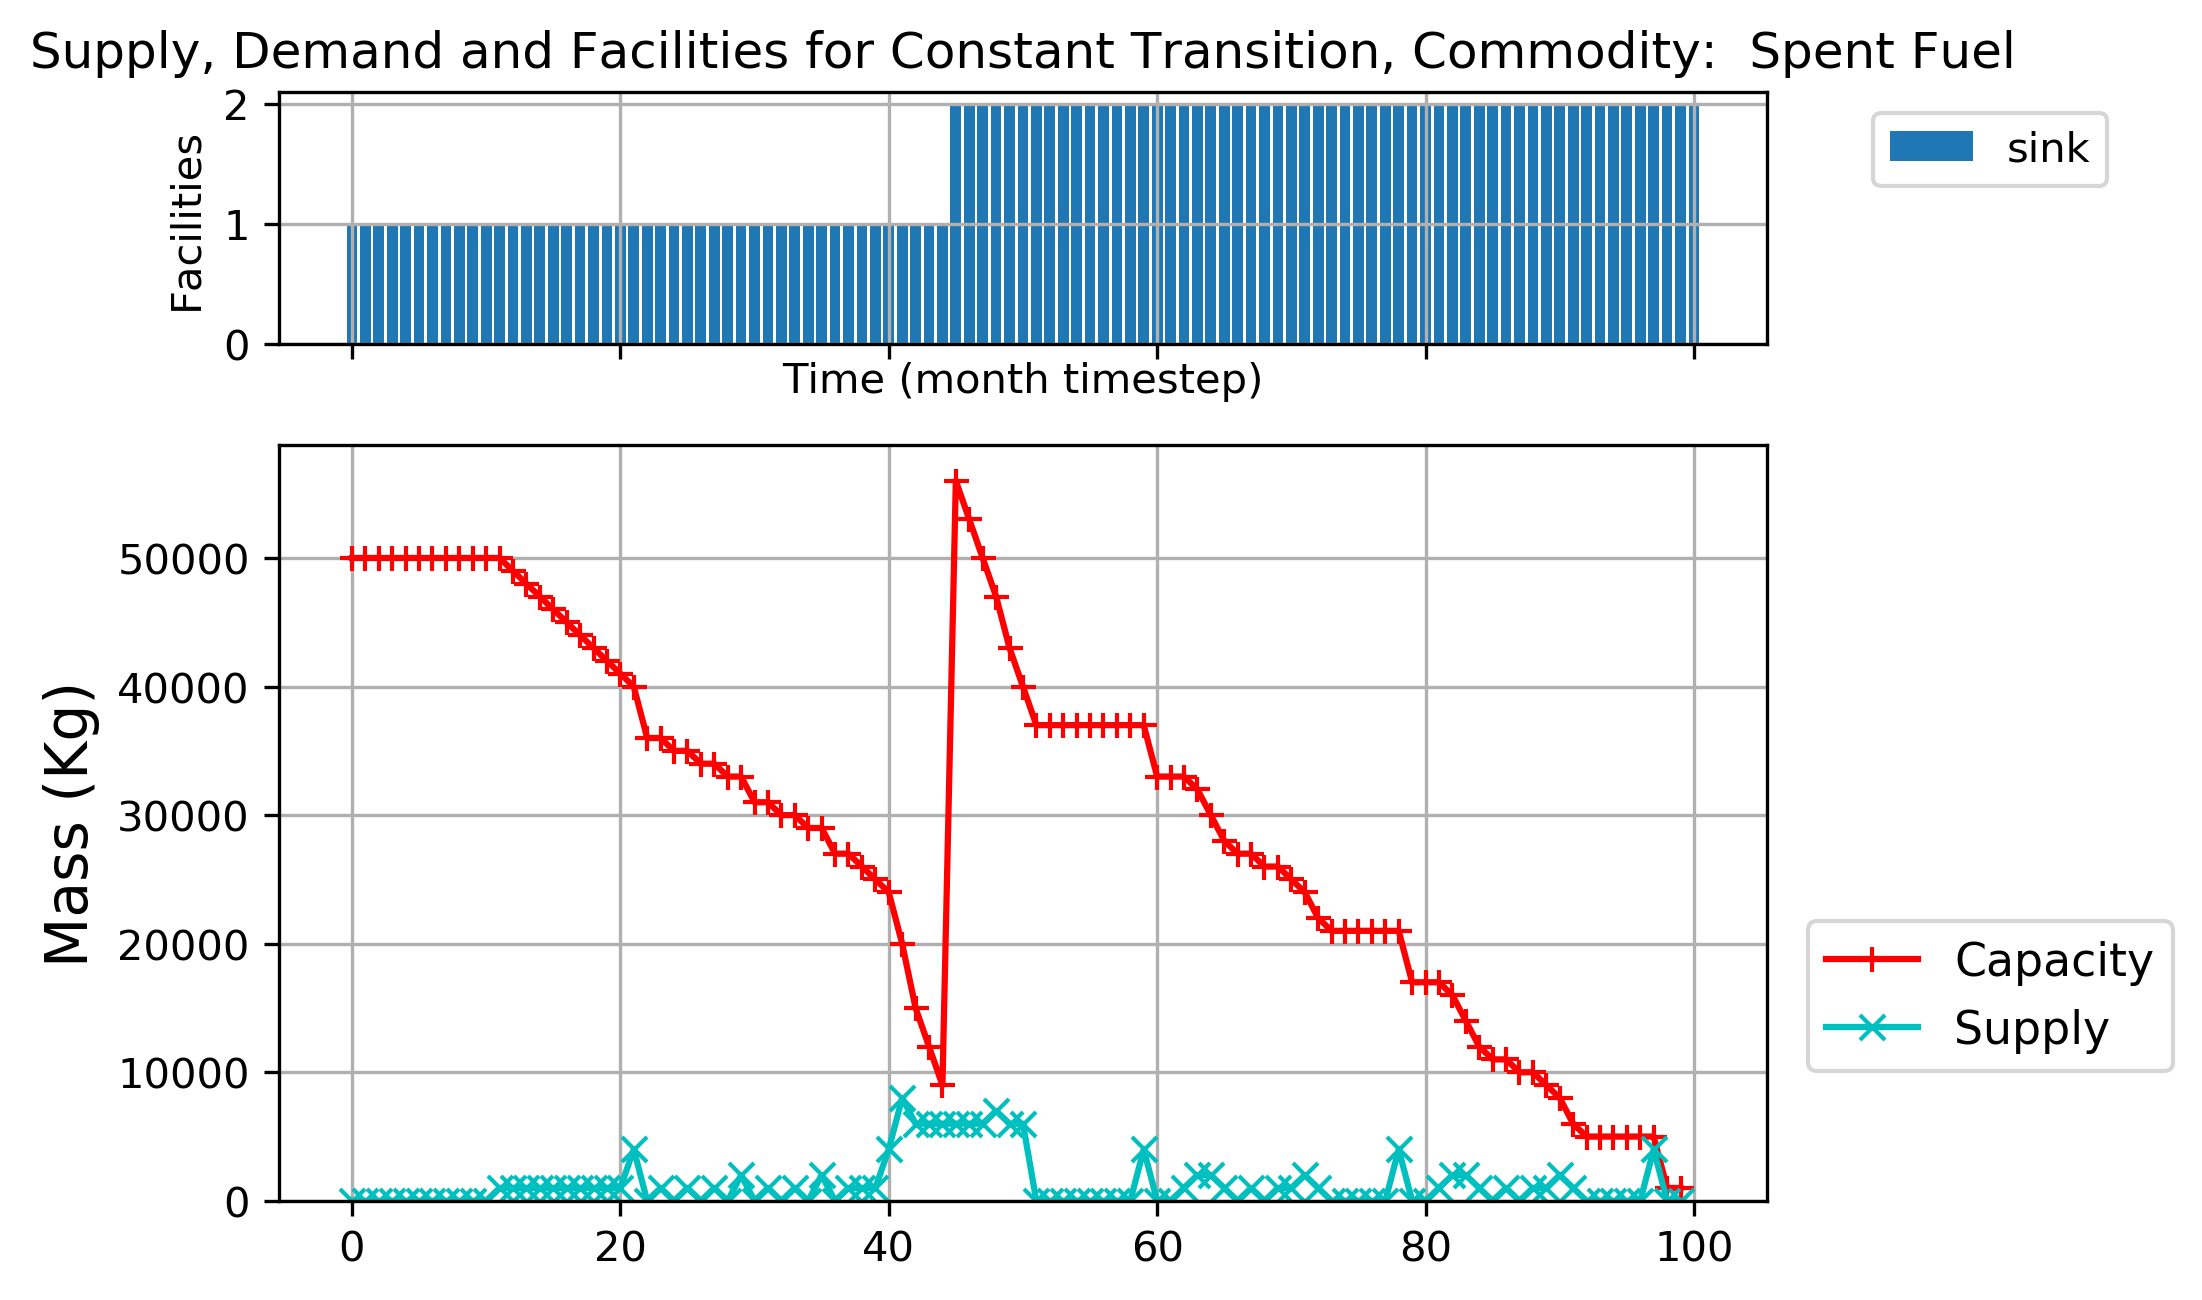
\includegraphics[width=\linewidth]{figures/constanttransition-spentfuel.png} 
            \caption{Spent Fuel is supplied by reactors and the capacity is provided by sink facilities.}
            \label{fig:constanttransition-spentfuel}
        \end{subfigure}
        \caption{Transition Scenario: Constant Power Demand of 10000MW}
    \end{figure}

    \subsection{Simple Transition Scenario Simulation: Linearly Increasing Demand}

    Figures \ref{fig:growingtransition-power}, \ref{fig:growingtransition-fuel},
    and \ref{fig:growingtransition-spentfuel} demonstrate the capability 
    of \deploy to deploy reactor and supporting facilities to meet the
    power demand and subsequently demanded secondary commodities 
    for a linearly increasing power demand. 
    This transition utilizes a smaller supply buffer compared to the constant 
    power case to minimize power undersupply.
    Table \ref{tab:transition-scenario-results} shows the number of 
    undersupplied timesteps. 
    In Figure \ref{fig:growingtransition-power}, there exist no time steps 
    in which the supply of power falls under demand, meeting the main 
    objective of \deploy. 
    
    \begin{figure}[]
        \centering
        \begin{subfigure}[t]{\textwidth}
        \centering
            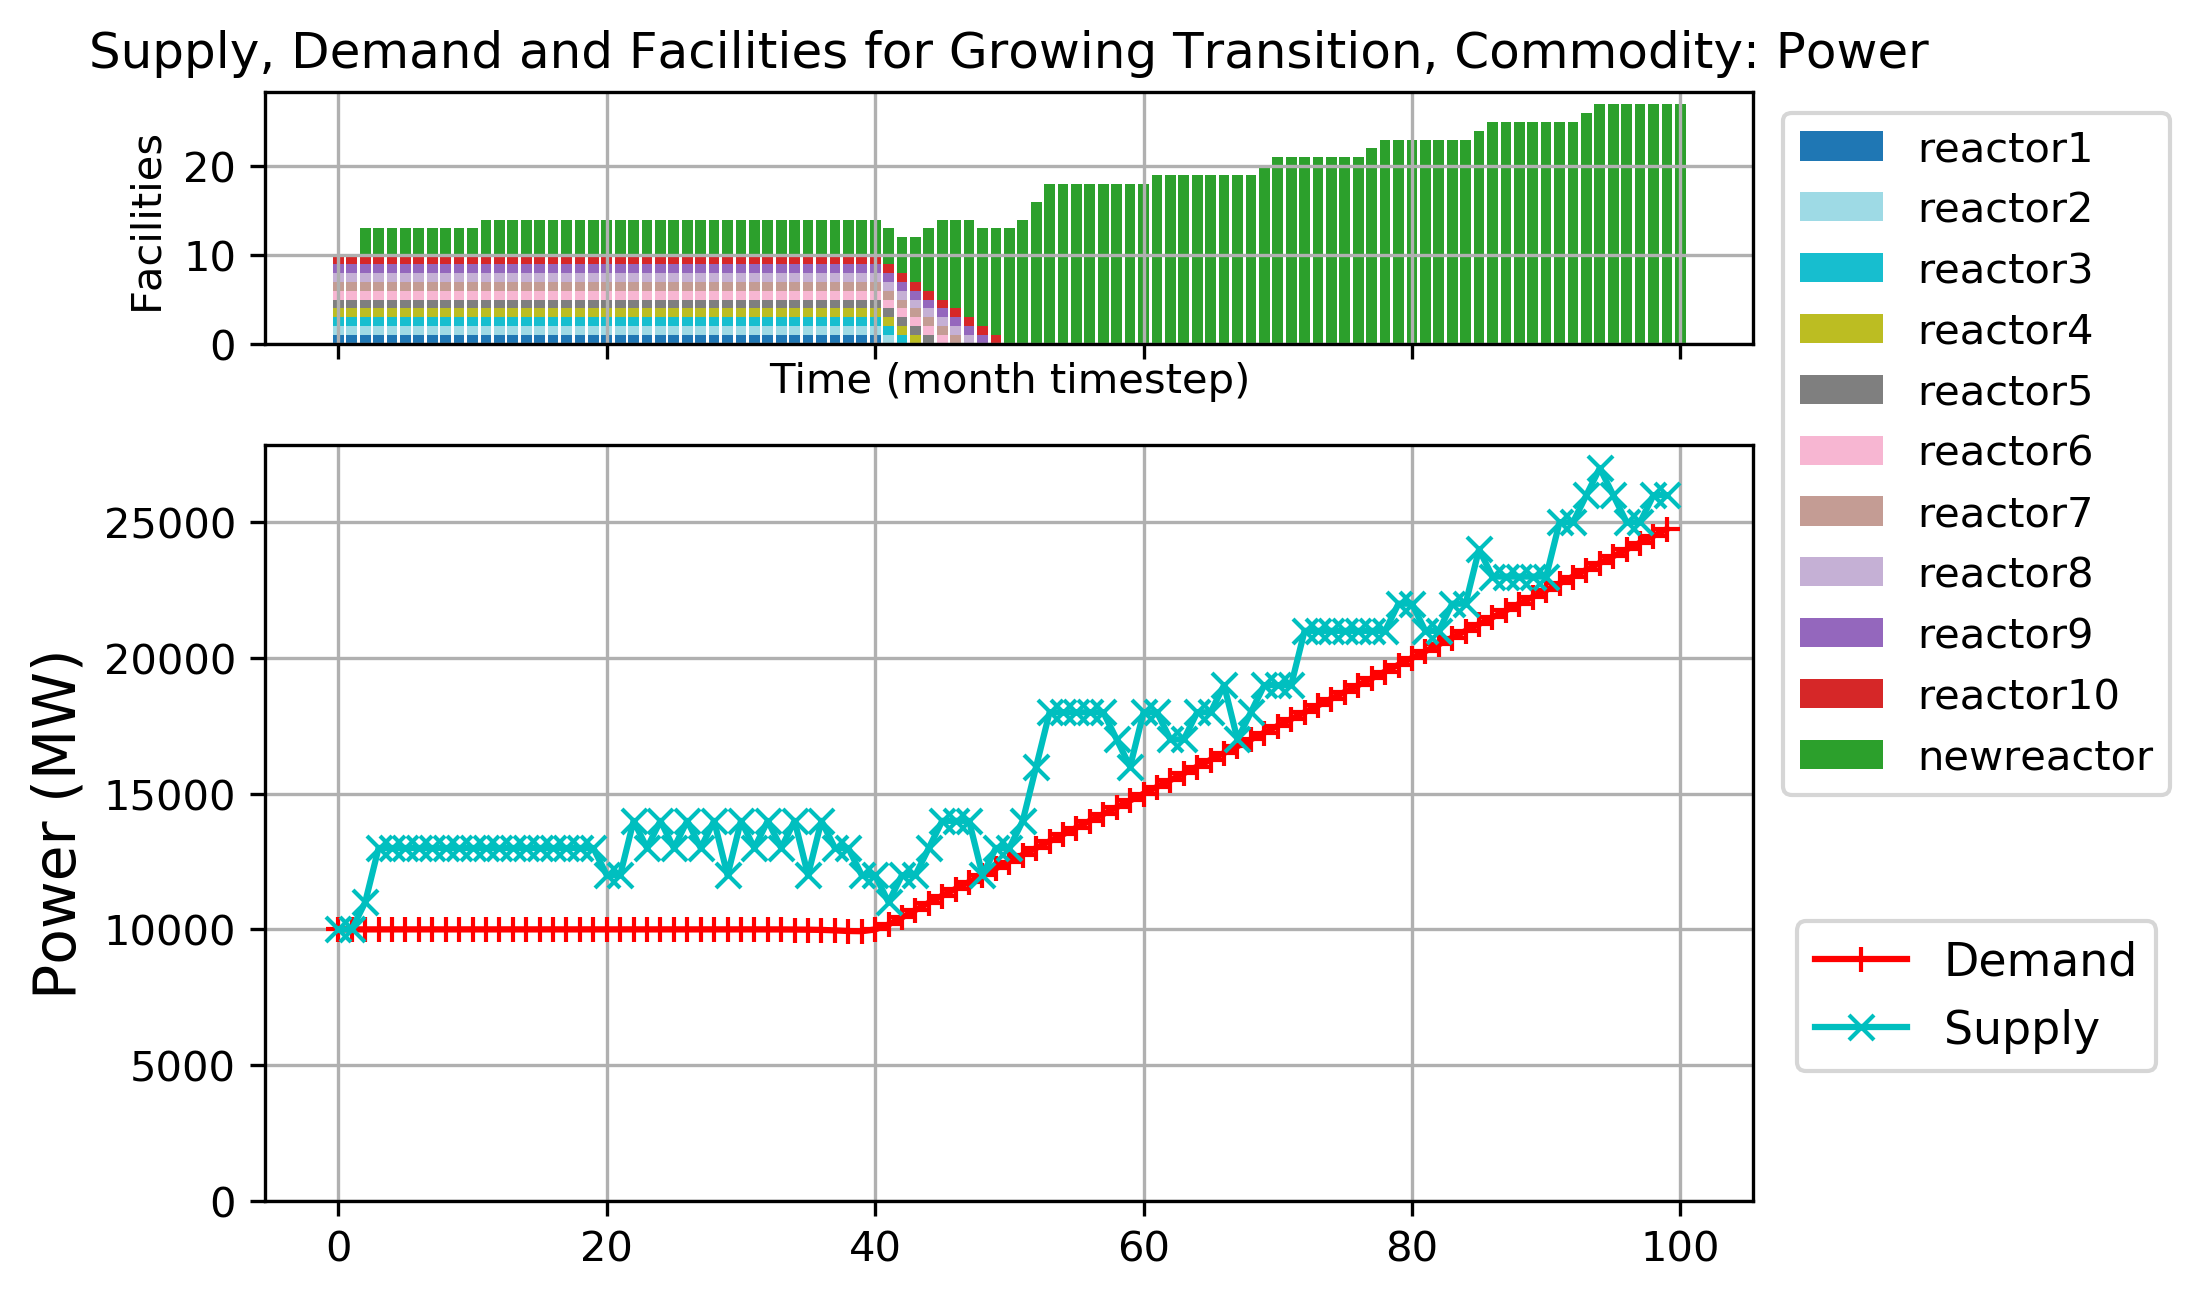
\includegraphics[width=0.7\linewidth]{figures/growingtransition-power.png} 
            \caption{The power demand is a user-defined equation and power is supplied by the reactors.}
            \label{fig:growingtransition-power}
        \end{subfigure}
        \begin{subfigure}[t]{0.6\textwidth}
            \centering
            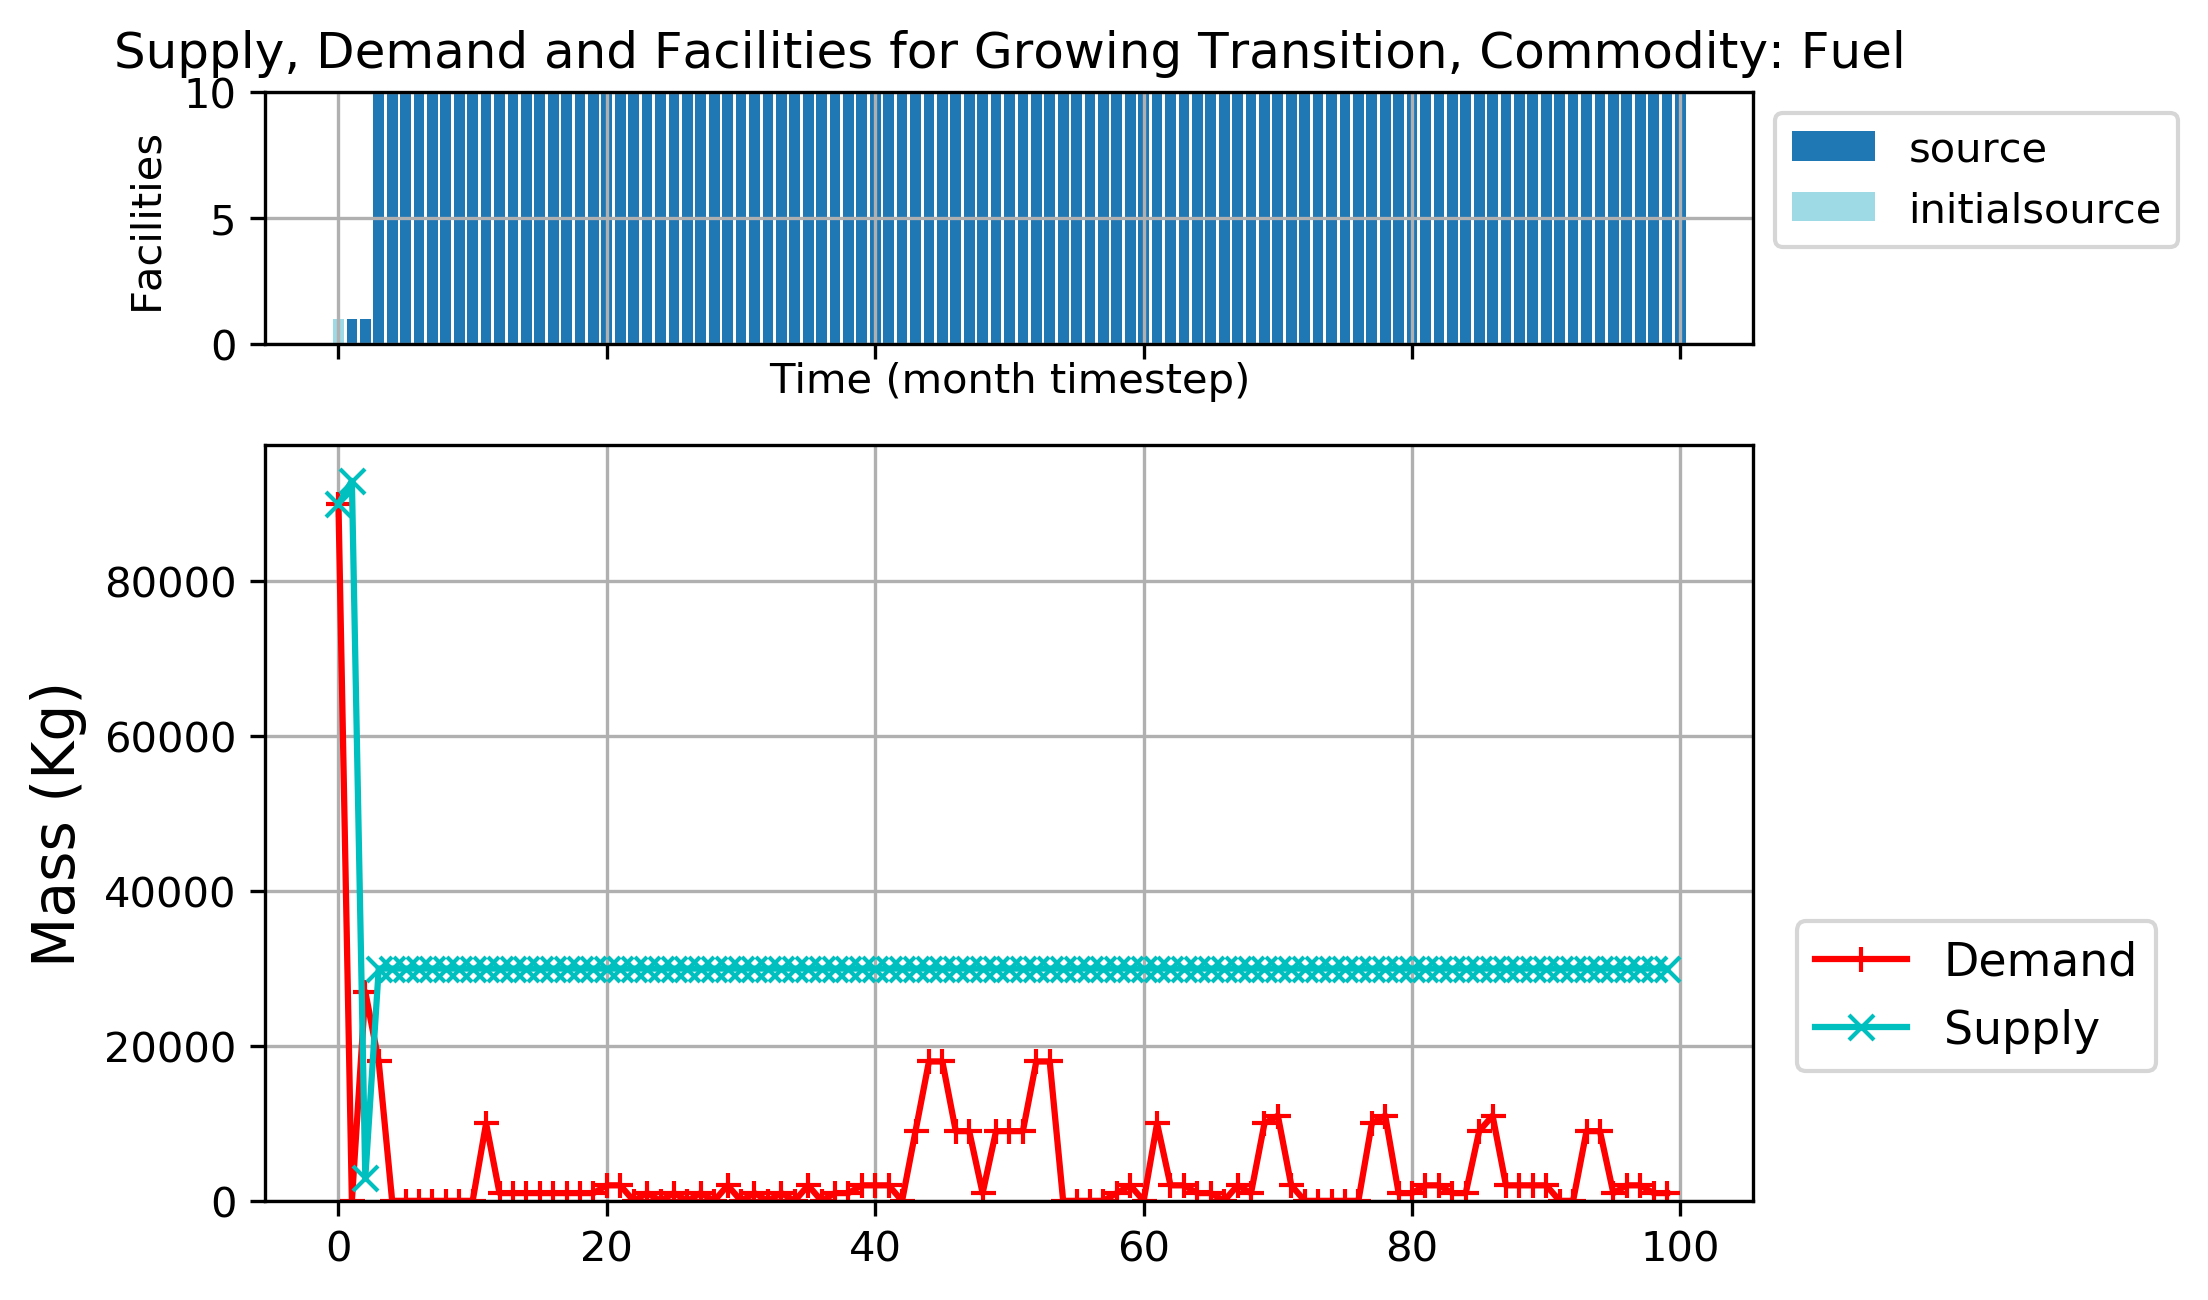
\includegraphics[width=\linewidth]{figures/growingtransition-fuel.png} 
            \caption{Fuel is demanded by reactors and supplied by source facilities.}
            \label{fig:growingtransition-fuel}
        \end{subfigure}
        \begin{subfigure}[t]{0.6\textwidth}
            \centering
            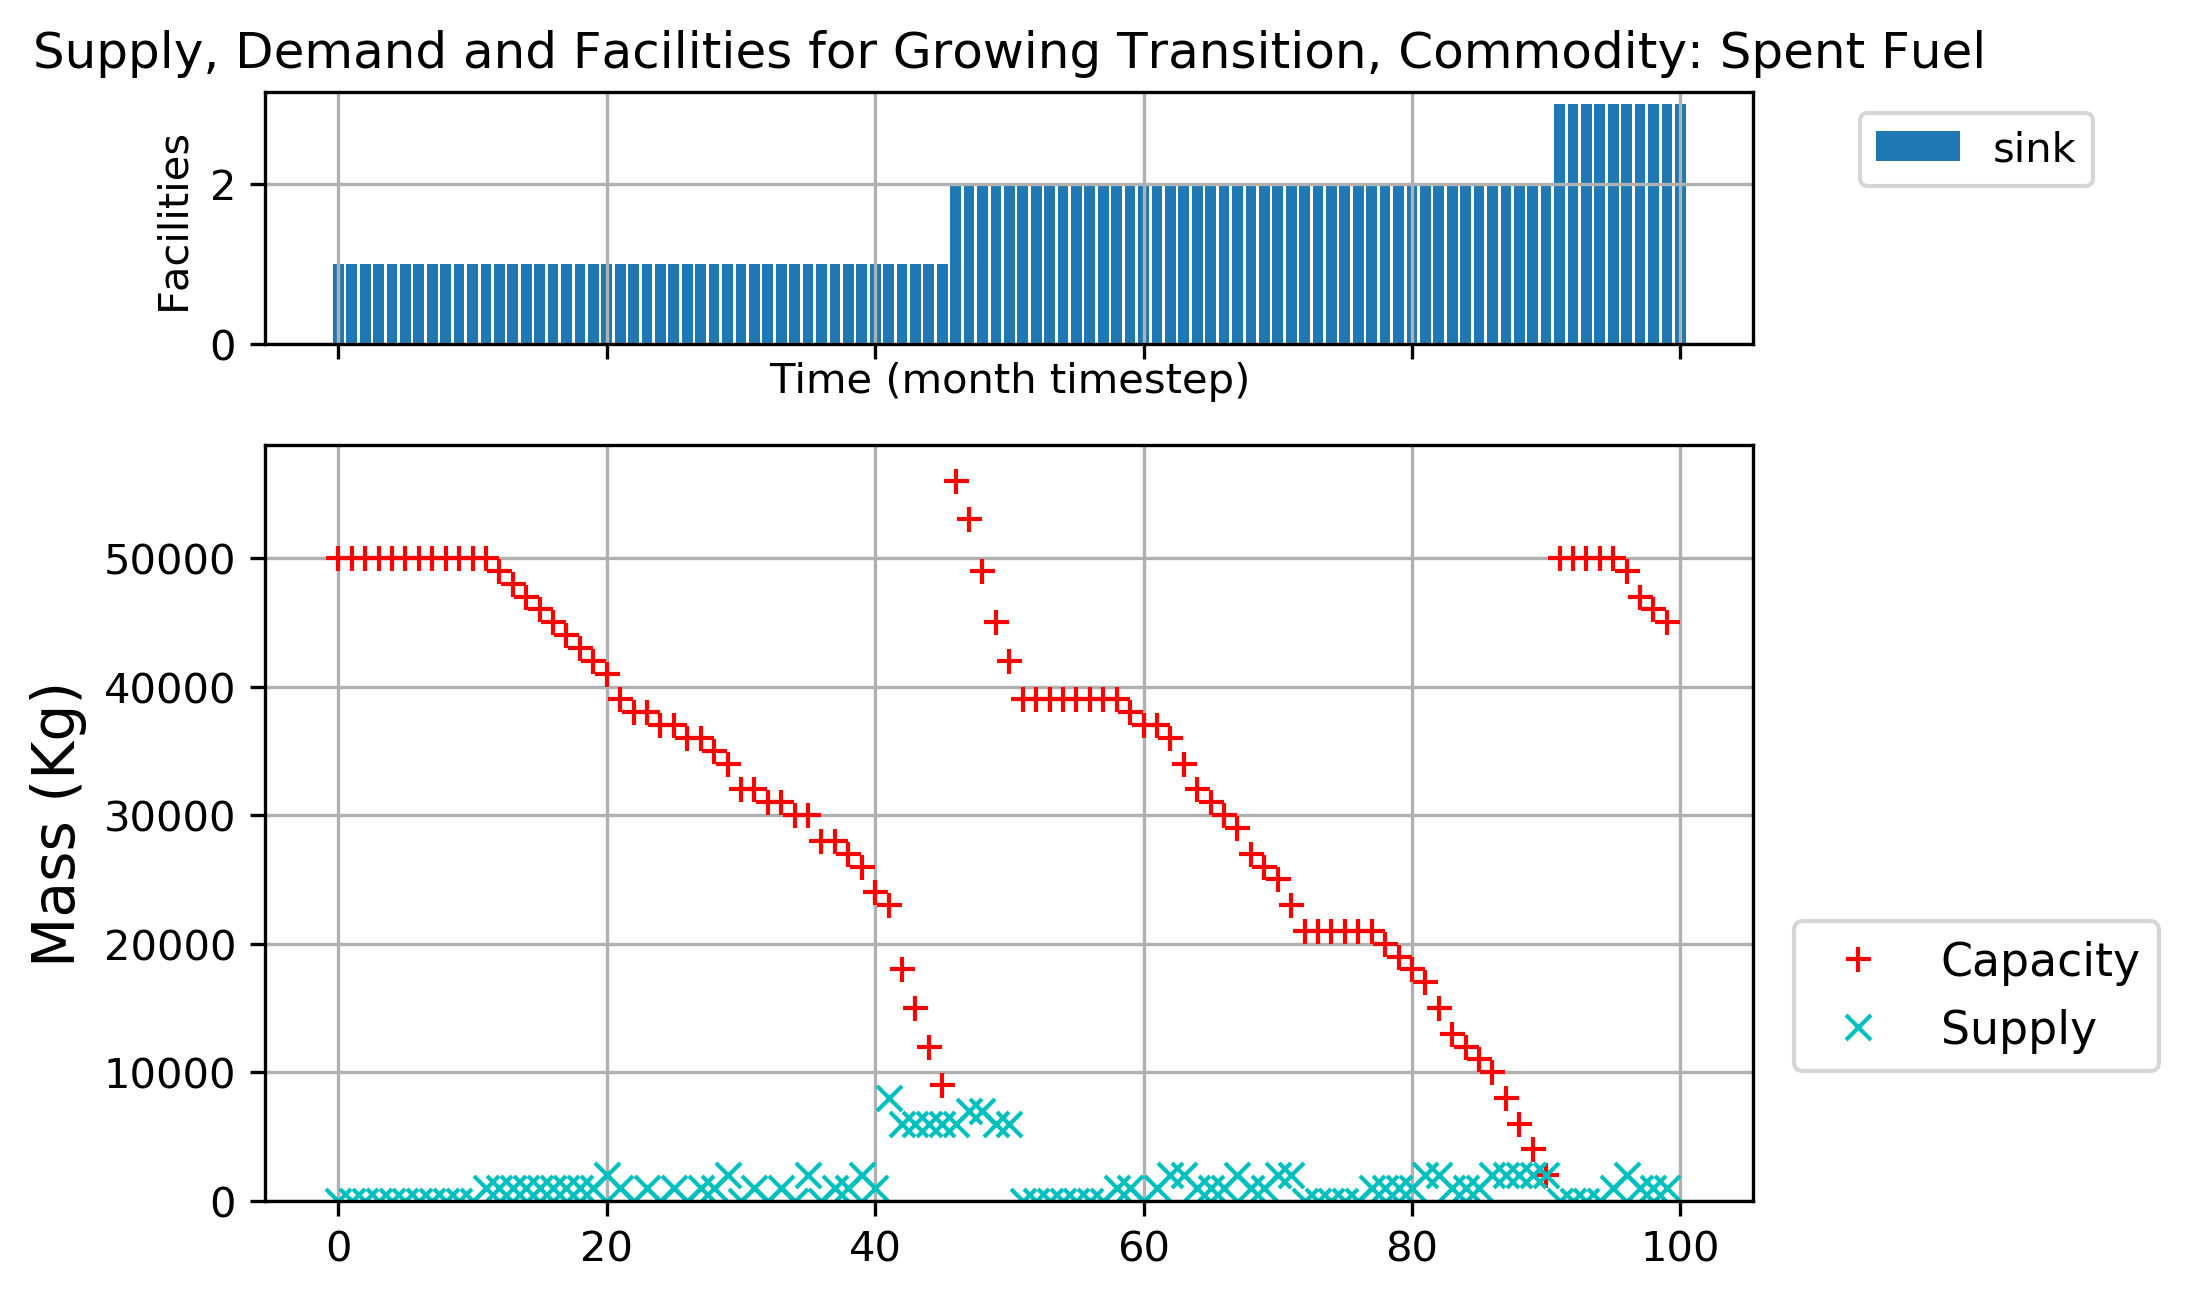
\includegraphics[width=\linewidth]{figures/growingtransition-spentfuel.png} 
            \caption{Spent Fuel is supplied by reactors and the capacity is provided by sink facilities.}
            \label{fig:growingtransition-spentfuel}
        \end{subfigure}
        \caption{Transition Scenario: Linearly Increasing Power Demand.}
    \end{figure}
    
    \subsection{Simple Transition Scenario Simulation: Sinusoidal Demand}
    Sinusoidal power demand is the reflection of power demand in 
    the real world where power usage is higher in the winter and summer
    and lower in the spring and fall. 
    Figures \ref{fig:sinetransition-power}, \ref{fig:sinetransition-fuel},
    and \ref{fig:sinetransition-spentfuel} demonstrate the capability 
    of \deploy to deploy reactor and supporting facilities to meet the
    power demand and subsequently demanded secondary commodities 
    for sinusoidal power demand. 
    Table \ref{tab:transition-scenario-results} shows the number of 
    undersupplied timesteps.
    
    For a sinusoidal power demand, the use of the 
    \texttt{holt-winters} method
    for predicting demand is more effective than the 
    \texttt{FFT} method used for the constant 
    and linearly increasing power demand transition scenarios. 
    This is because the \texttt{holt-winters} method excels in
    forecasting data points for repetitive seasonal series of data. 
    
    \begin{figure}[]
        \centering
        \begin{subfigure}[t]{\textwidth}
        \centering
            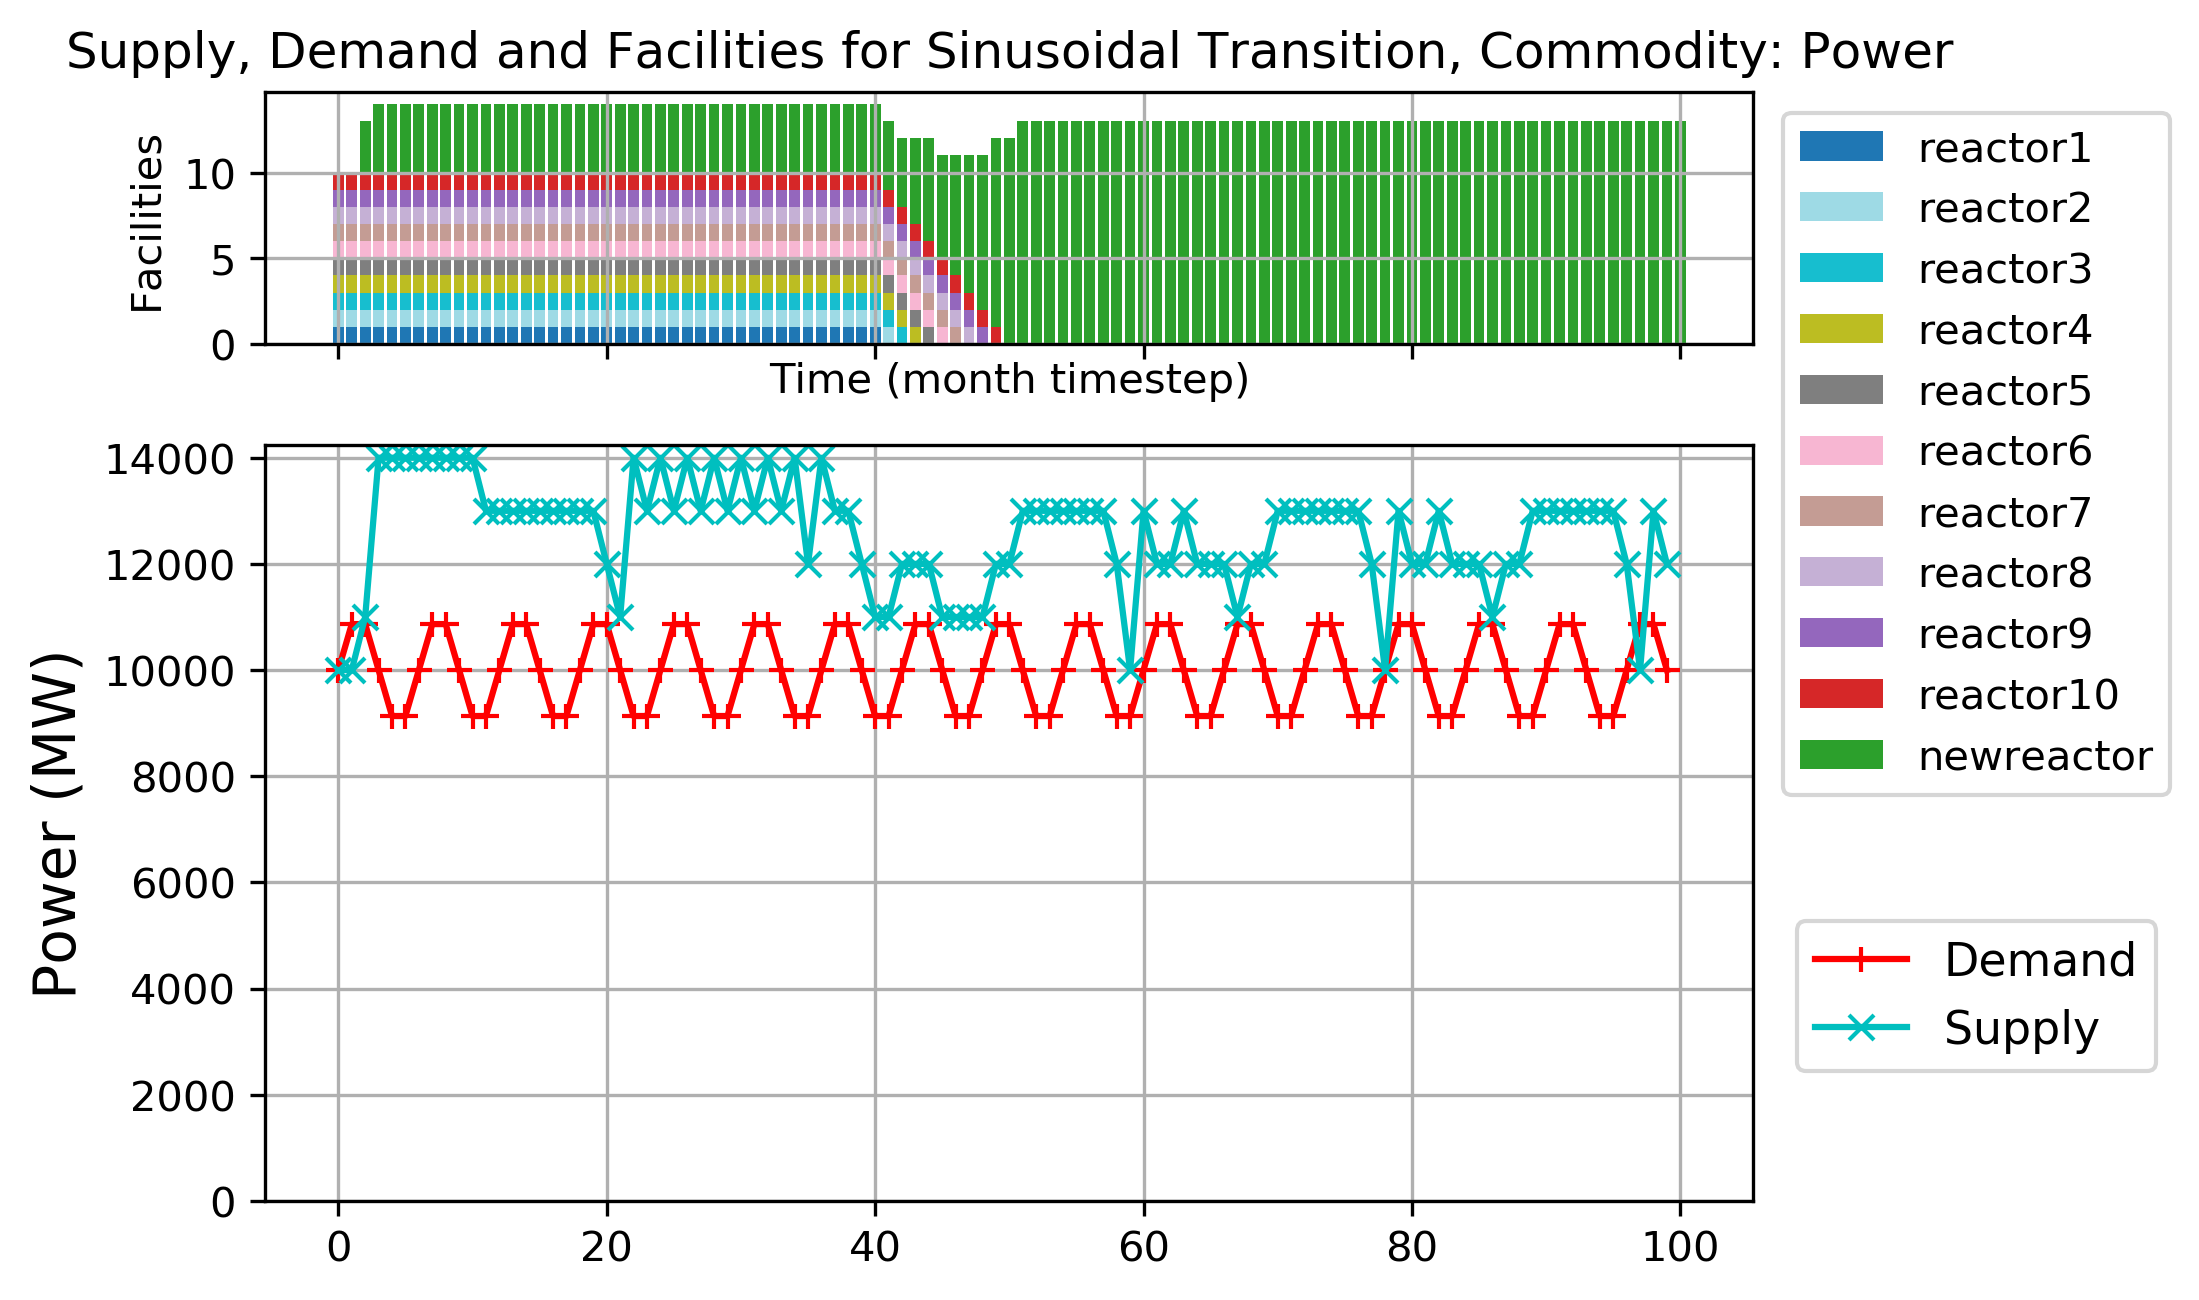
\includegraphics[width=0.7\linewidth]{figures/sinetransition-power.png} 
            \caption{The power demand is a user-defined equation and power is supplied by the reactors.}
            \label{fig:sinetransition-power}
        \end{subfigure}
        \begin{subfigure}[t]{0.6\textwidth}
            \centering
            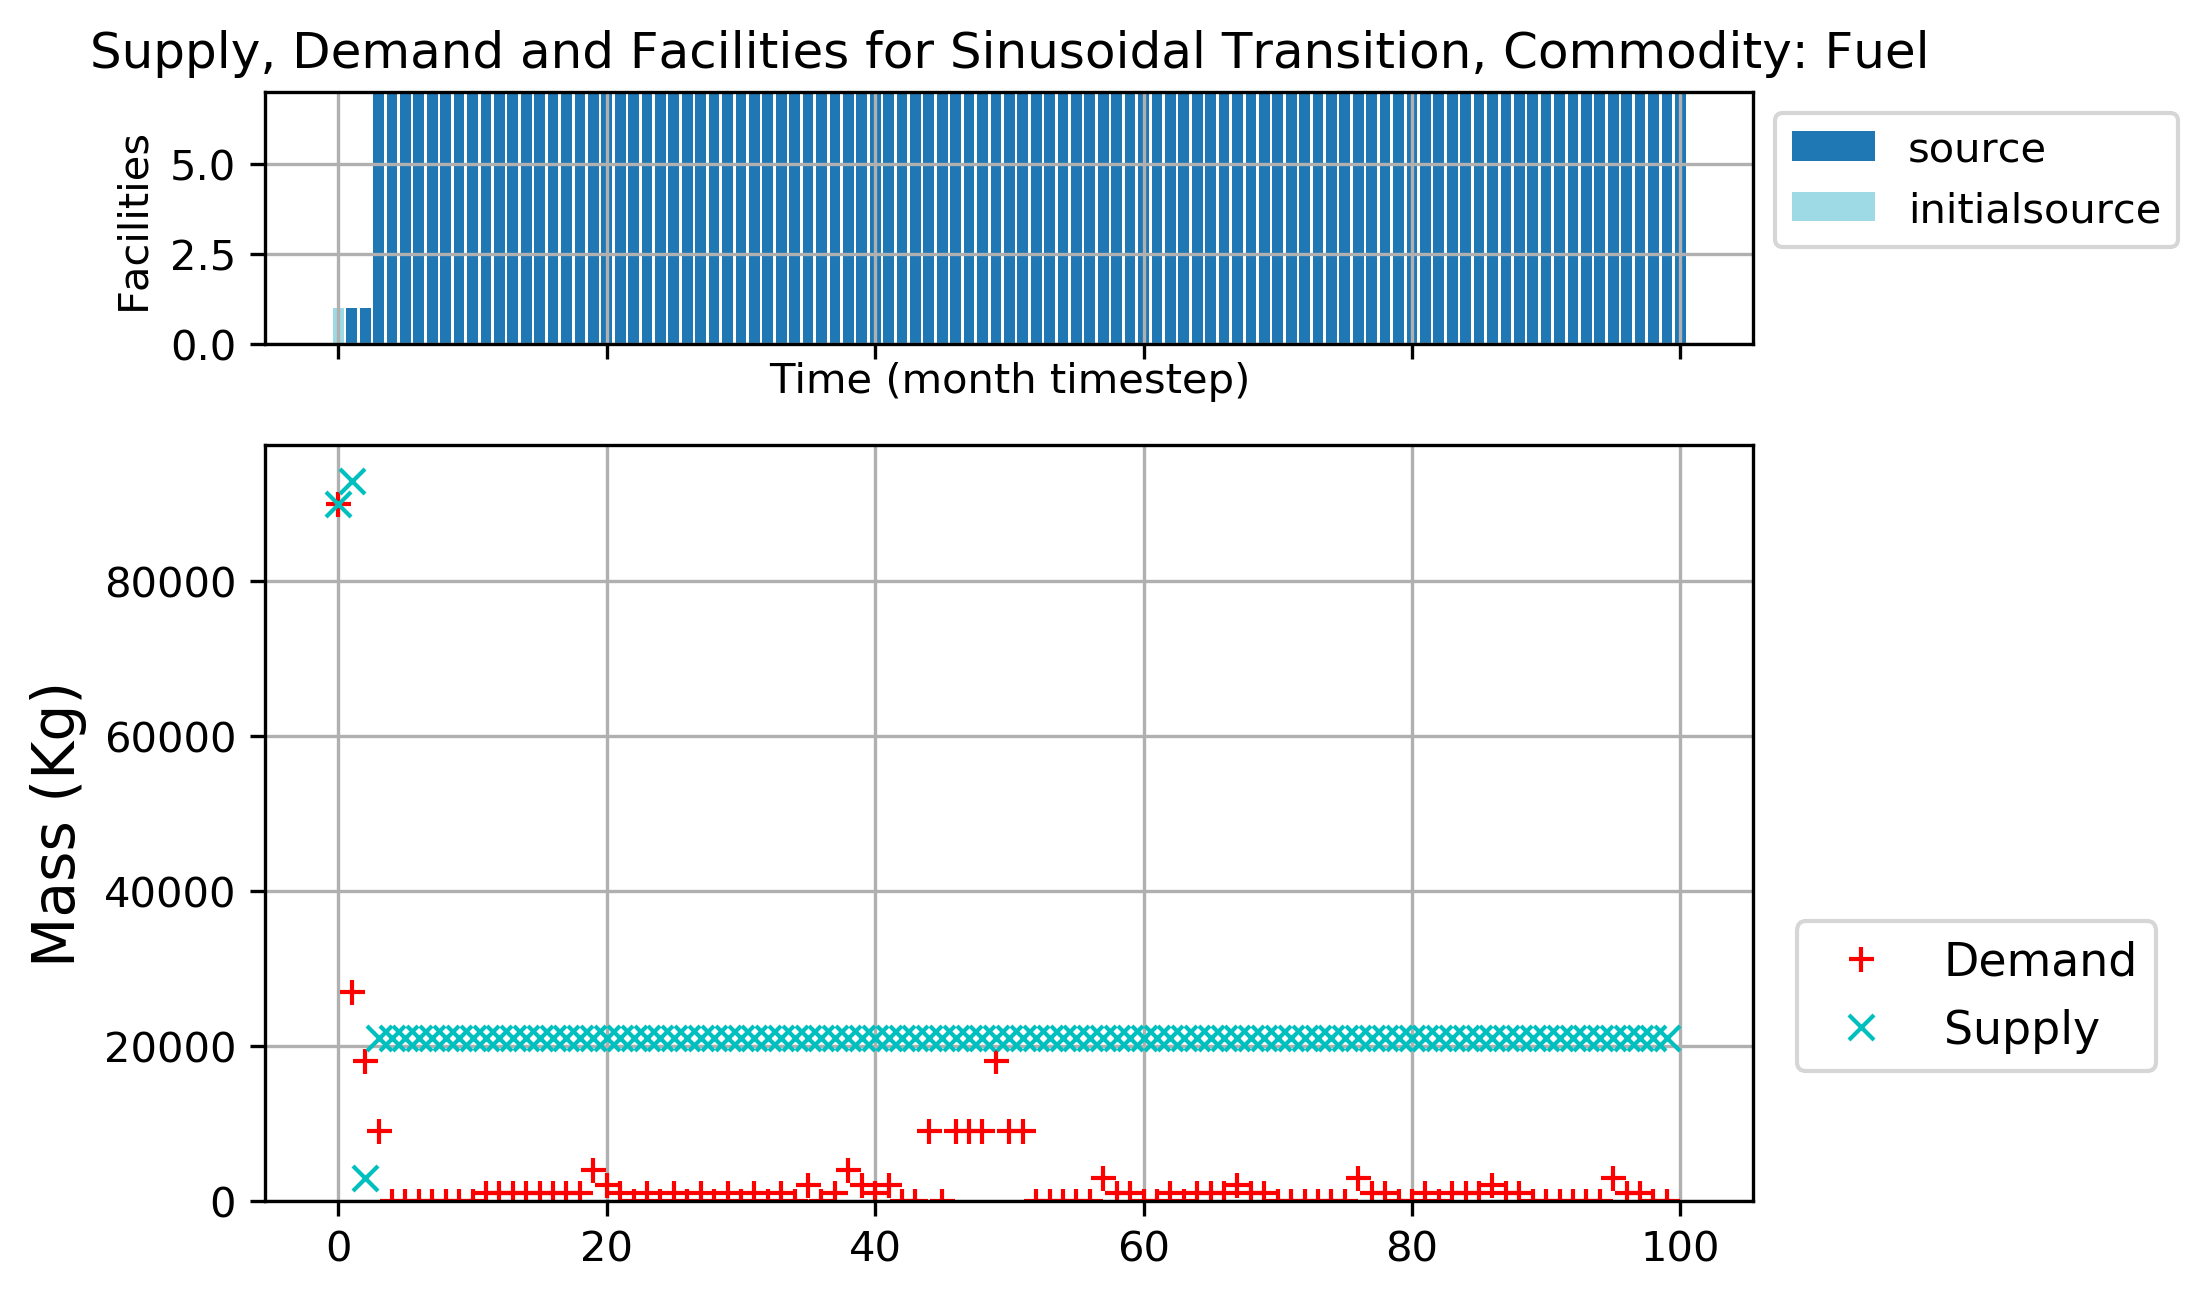
\includegraphics[width=\linewidth]{figures/sinetransition-fuel.png} 
            \caption{Fuel is demanded by reactors and supplied by source facilities.}
            \label{fig:sinetransition-fuel}
        \end{subfigure}
        \begin{subfigure}[t]{0.6\textwidth}
            \centering
            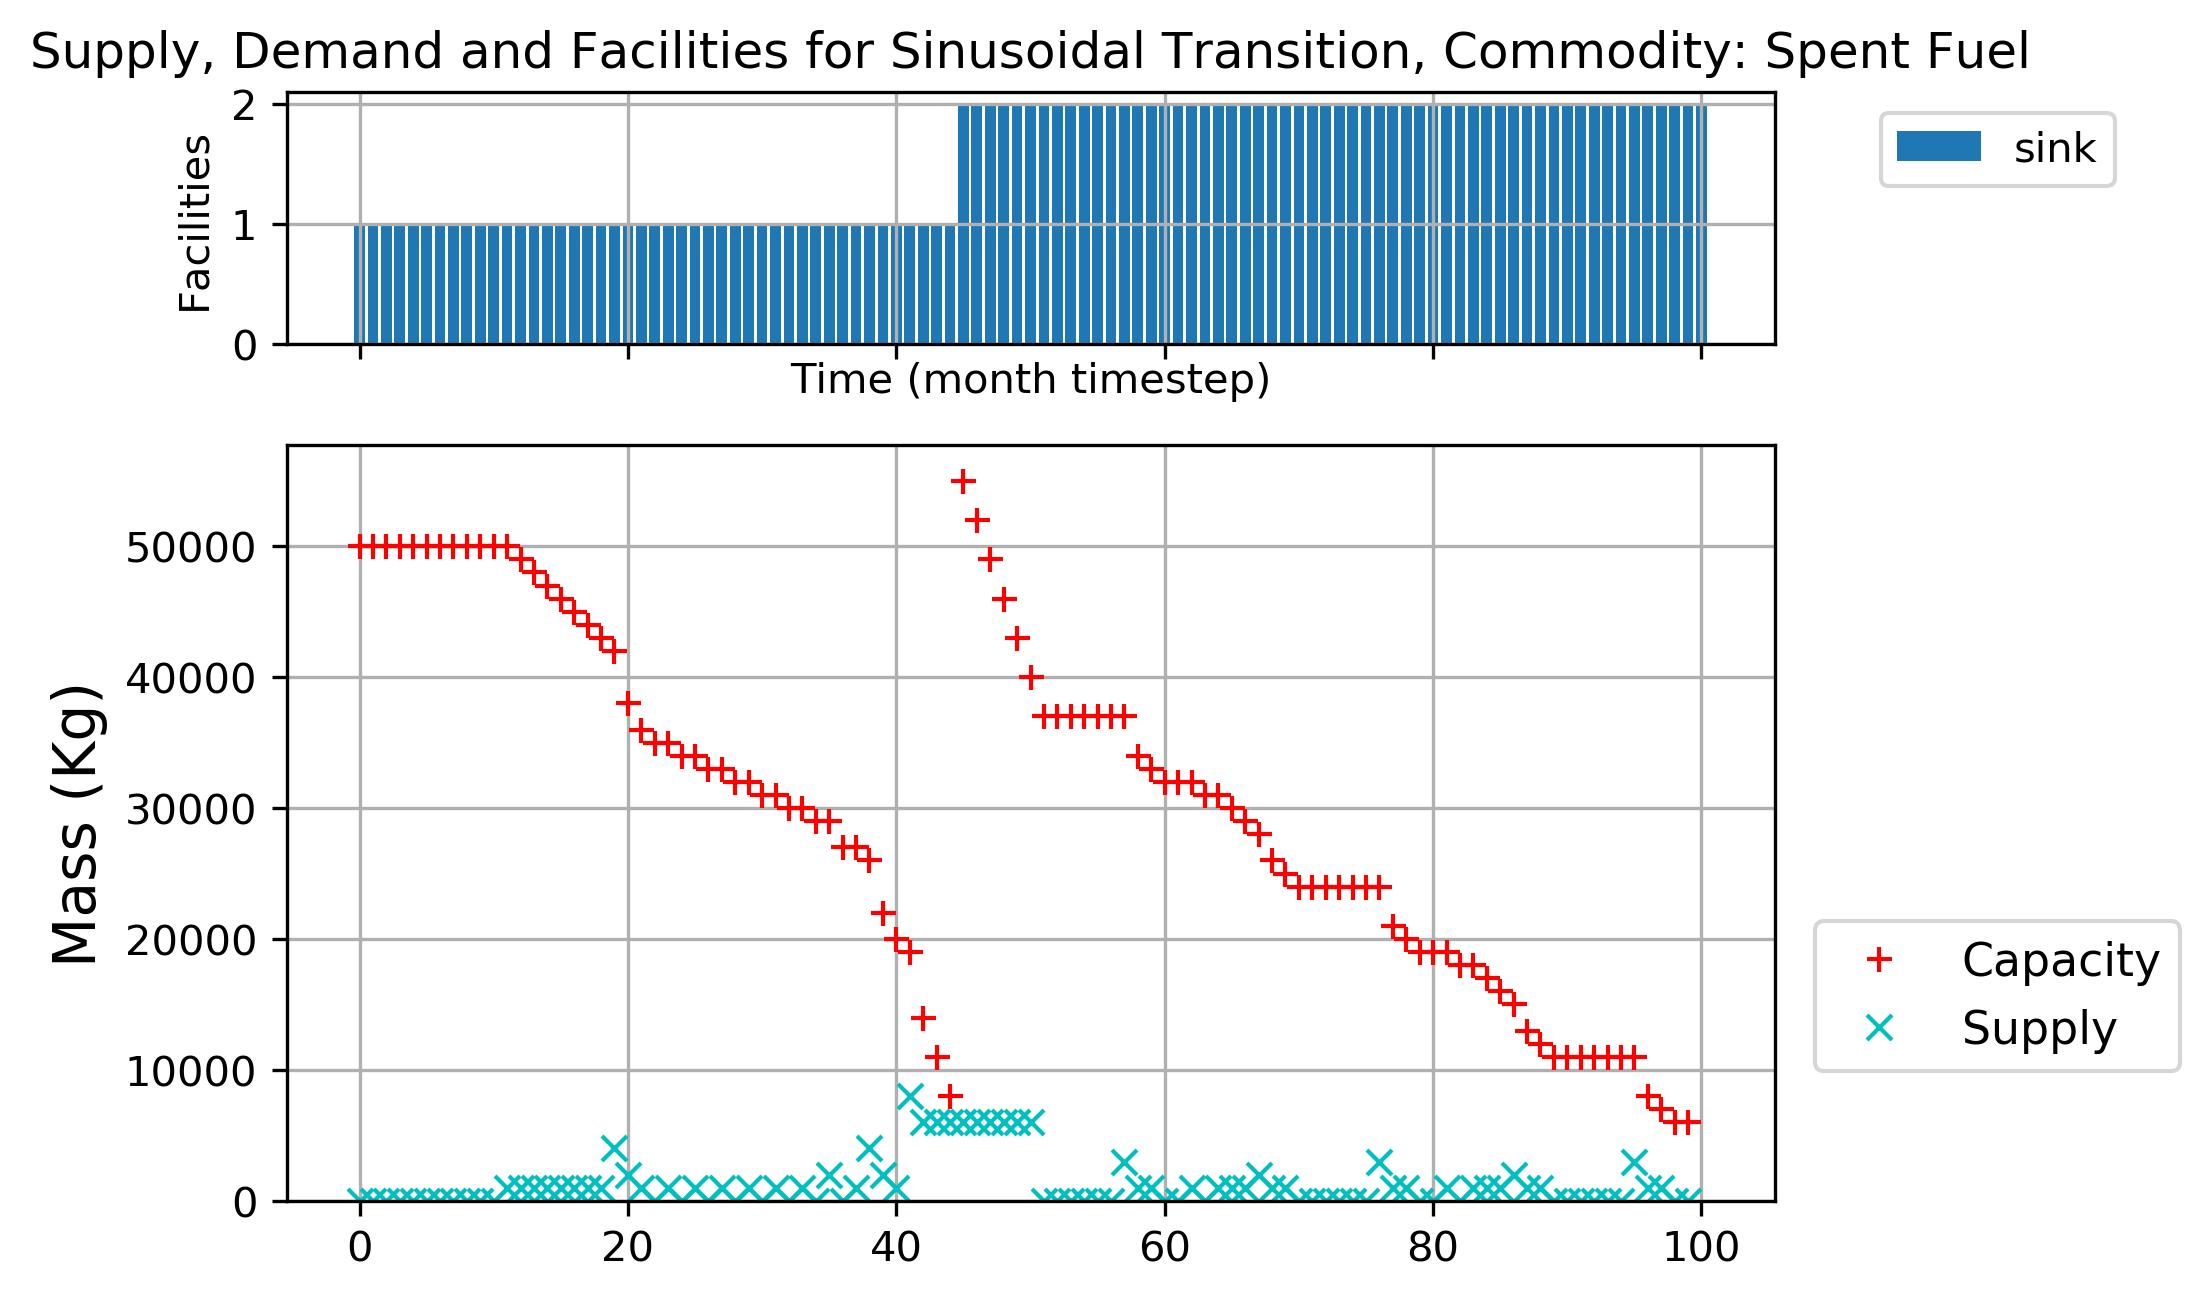
\includegraphics[width=\linewidth]{figures/sinetransition-spentfuel.png} 
            \caption{Spent Fuel is supplied by reactors and the capacity is provided by sink facilities.}
            \label{fig:sinetransition-spentfuel}
        \end{subfigure}
        \caption{Transition Scenario: Sinusoidal Power Demand}
    \end{figure}

    \begin{table}[]
        \centering
        \caption {Undersupply results for each commodity in each simple transition scenario}
        \label{tab:transition-scenario-results}
            \footnotesize
            \begin{tabular}{l|rr}	
                \hline
                \textbf{Basic Transition Scenario}    & \textbf{Commodity}    & \textbf{No. of undersupply timesteps} \\ \hline
                \multirow{2}{*}{\textbf{Constant Power}} & Fuel & 1 \\ 
                                                         & Power & 0 \\ 
                                                         & Spent Fuel & 0 \\ \hline
                \multirow{2}{*}{\textbf{Linearly Increasing Power}} & Fuel & 1 \\ 
                                                         & Power & 0 \\ 
                                                         & Spent Fuel & 0 \\ \hline
                \multirow{2}{*}{\textbf{Sinusoidal Power}} & Fuel & 1 \\ 
                                                         & Power & 1 \\ 
                                                         & Spent Fuel & 0 \\ \hline
                \end{tabular}
    \end{table}

\section{\deploy Demonstration of EG01-30 Transition Scenario} 
\label{sec:eg01-30}
Figure \ref{fig:30flow} shows the setup of facilities and mass flows 
for EG01-30 in \Cyclus. 
In the EG01-30 transition scenario, the initial LWR fleet 
progressively decommissions at the 80-year mark,
after which \deploy deploys \glspl{SFR} and \gls{MOX} \glspl{LWR} to 
meet a linearly increasing power demand. 
Transuranic elements from the spent fuel are recycled to 
produce \gls{MOX} \gls{LWR} and \gls{SFR} fuel. 
The power demand equation (t represents a month): 
\begin{align}
    P(t) = 60000 + \frac{250t}{12}\ MW
\end{align}

\begin{figure}[]
    \centering
    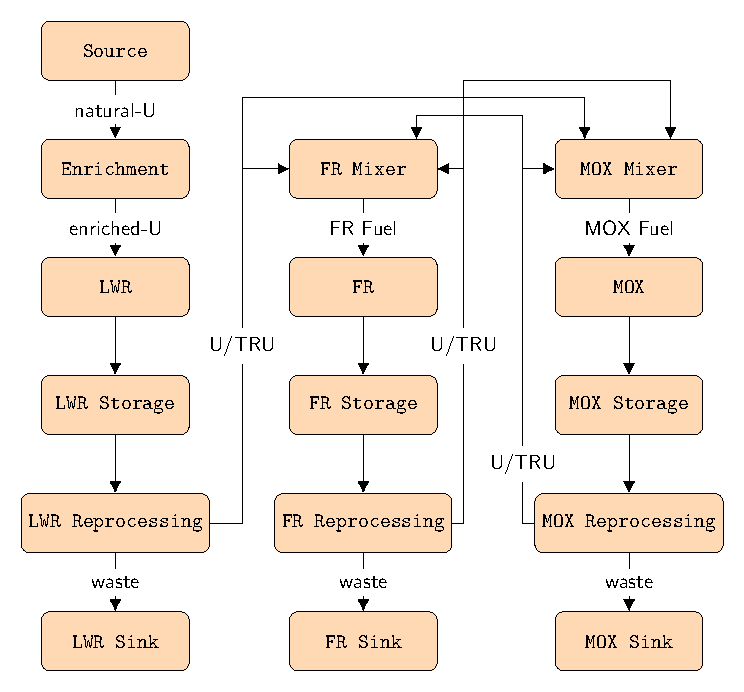
\includegraphics[width=0.55\linewidth]{30flow.pdf} 
    \caption{Facility and mass flow for EG01-30 transition scenario.}
    \label{fig:30flow}
\end{figure}

To determine the optimal \deploy parameters to minimize 
power undersupply in the EG01-30 \Cyclus 
transition scenario, a comparison study of prediction 
methods and power supply buffer sizes was conducted. 

\subsection{Comparison of Prediction Methods}
We ran EG01-30 transition scenarios with different prediction 
methods to determine the prediction method that best minimizes 
power undersupply. 
In Figure \ref{fig:eg30under}, the \texttt{fft} method has
the smallest and least number of crosses, 
demonstrating that it performs the best at minimizing 
undersupply of all commodities.
Thus, it is the best prediction method for this transition 
scenario simulation. 

% update these figures to actually be 30
\begin{figure}[]
	\centering
	\begin{subfigure}[t]{1\textwidth}
		\centering
		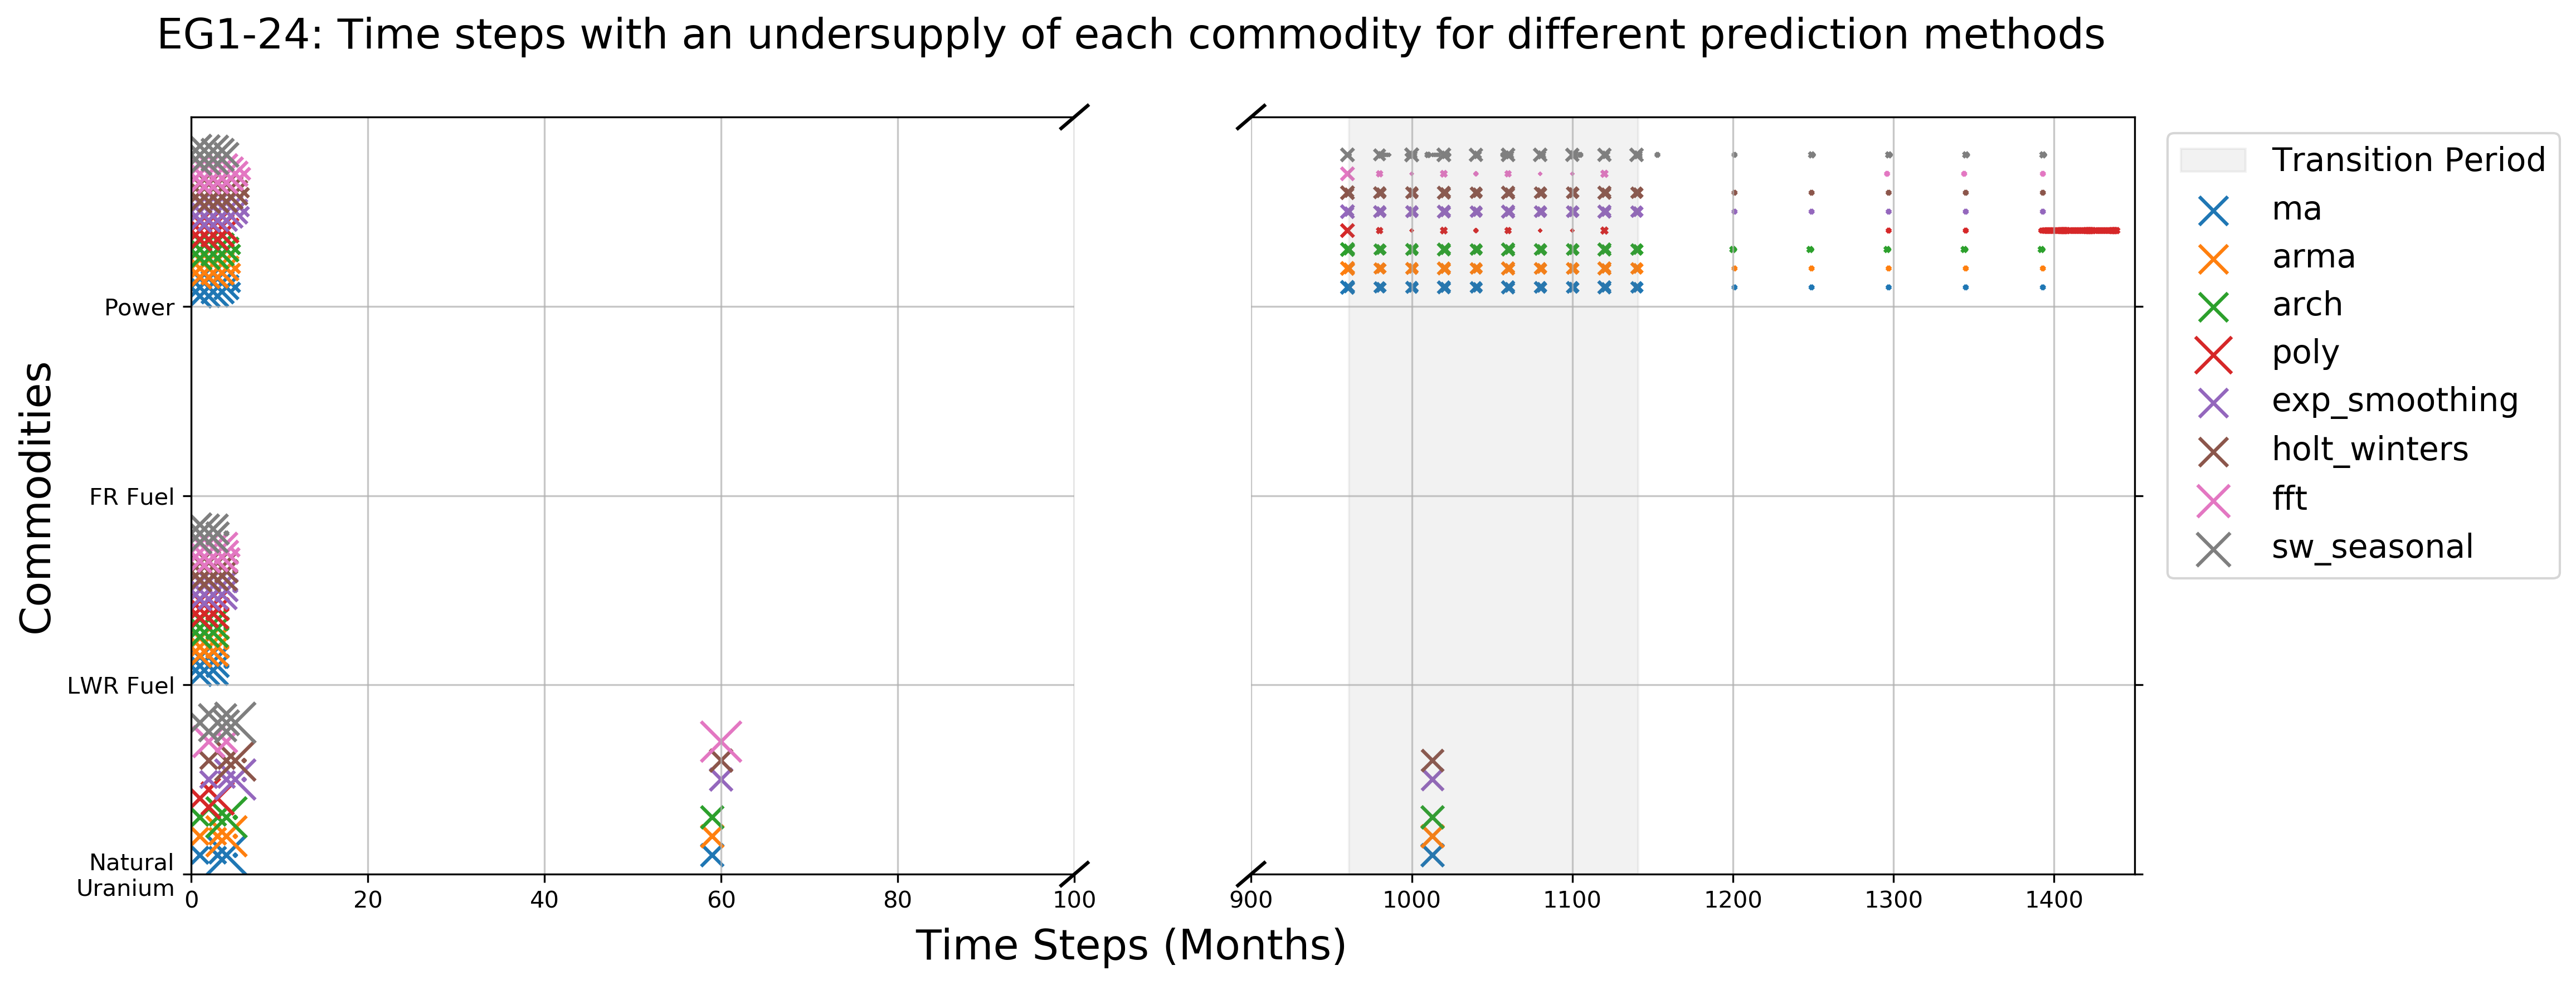
\includegraphics[width=\linewidth]{eg30-undersupply.png} 
		\caption{Time dependent undersupply of commodities in simulation }
		\label{fig:30undersupply}
	\end{subfigure}
	\vspace{1cm}
	\begin{subfigure}[t]{1\textwidth}
		\centering
		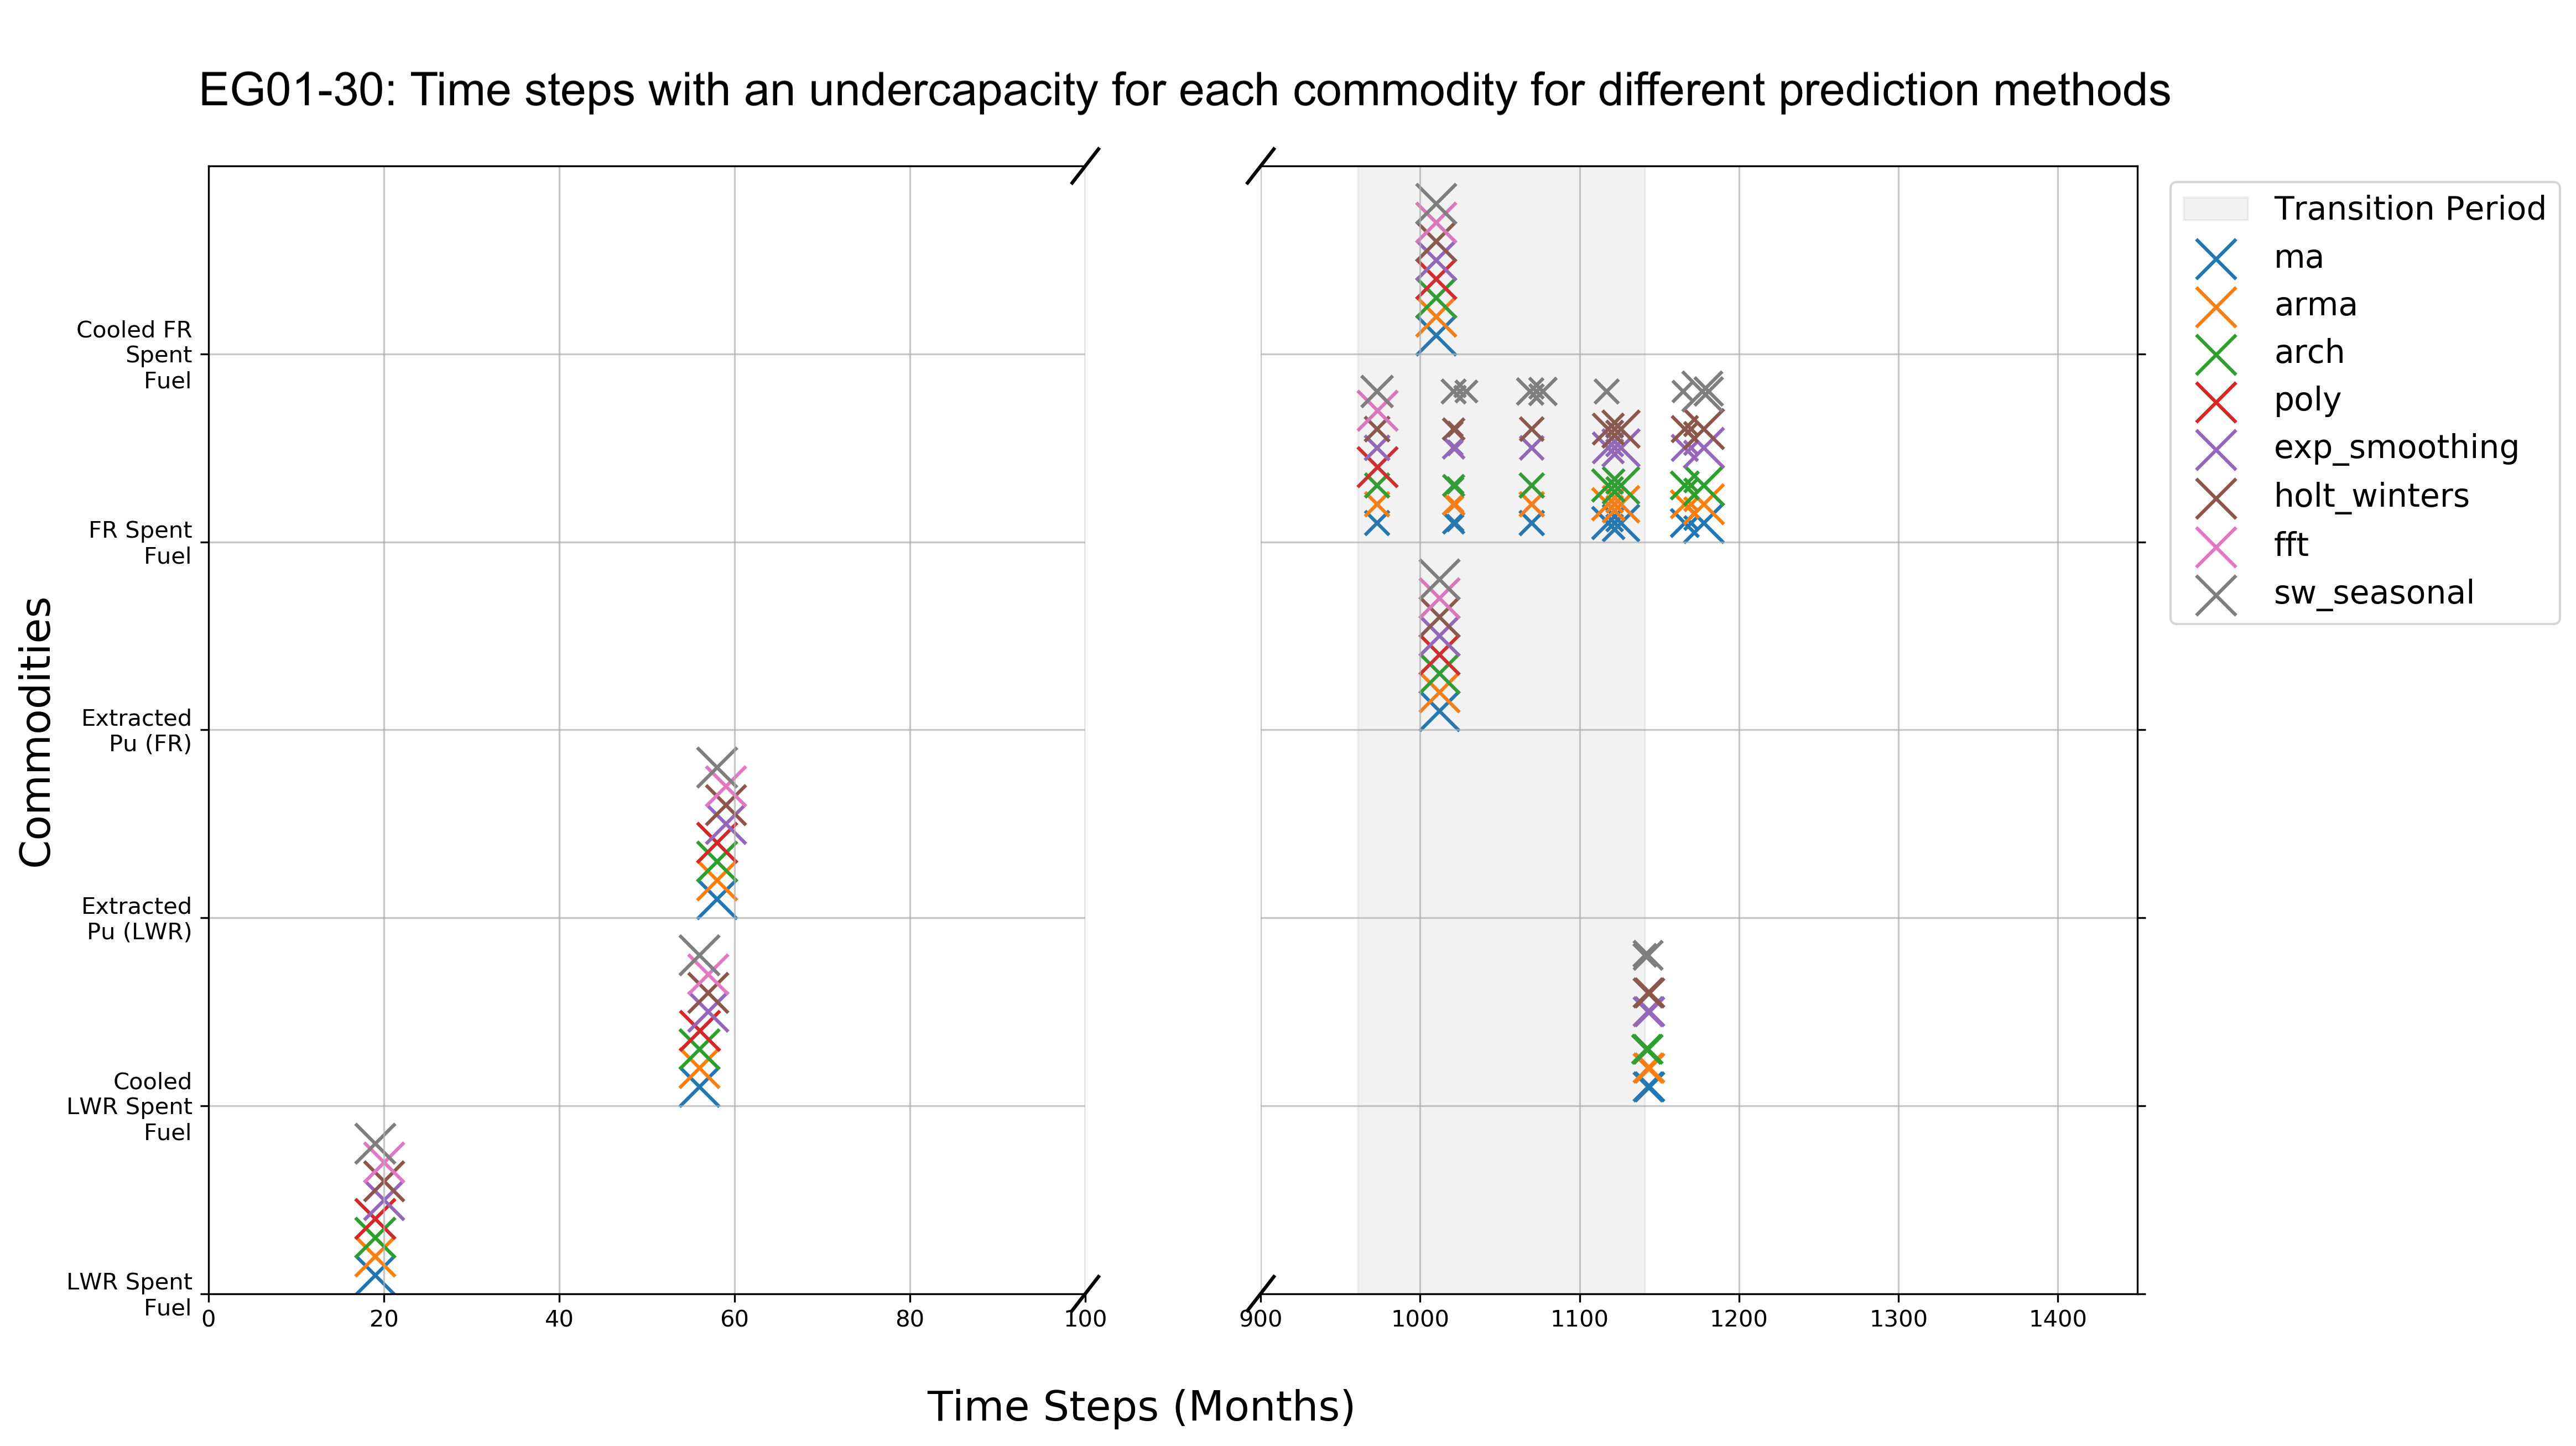
\includegraphics[width=\linewidth]{eg30-undercapacity.png} 
		\caption{Time dependent under capacity of commodities in simulation }
		\label{fig:30undercapacity}
	\end{subfigure}
	\hfill
	\caption{
	EG01-30 Transition Scenario with Linearly Increasing Power Demand:
	Each cross represent a time step in which there is undersupply 
	or under capacity of each commodity for varying prediction methods. 
    The size of each cross is proportional on the size of the undersupply.
    Larger crosses correspond to larger undersupply.}
	\label{fig:eg30under}
\end{figure}

\subsection{Comparison of Power Buffer Sizes}
For the EG01-30 linearly increasing power demand 
transition scenario, the power buffer size is varied. 
Figure \ref{fig:eg30-bufplot} and Table \ref{tab:buff_size} 
show that with increased buffer size, the number of 
power undersupply time steps decreases. 
The cumulative undersupply is the smallest for a buffer 
size of 8000MW.  
As seen from Figure \ref{fig:eg30-dotplot}, these undersupply time 
steps occur at the beginning of the simulation and for one 
time step when the transition begins. 
This is expected since without time series data 
at the beginning of the simulation, \deploy takes a few 
time steps to collect time series data about power demand 
to predict and start deploying reactor and supporting 
fuel cycle facilities. 
Therefore, a buffer of 8000MW minimizes 
the power undersupply for the EG01-EG30 transition scenario.

\begin{figure}[]
	\centering
	\begin{subfigure}[t]{\textwidth}
		\centering
		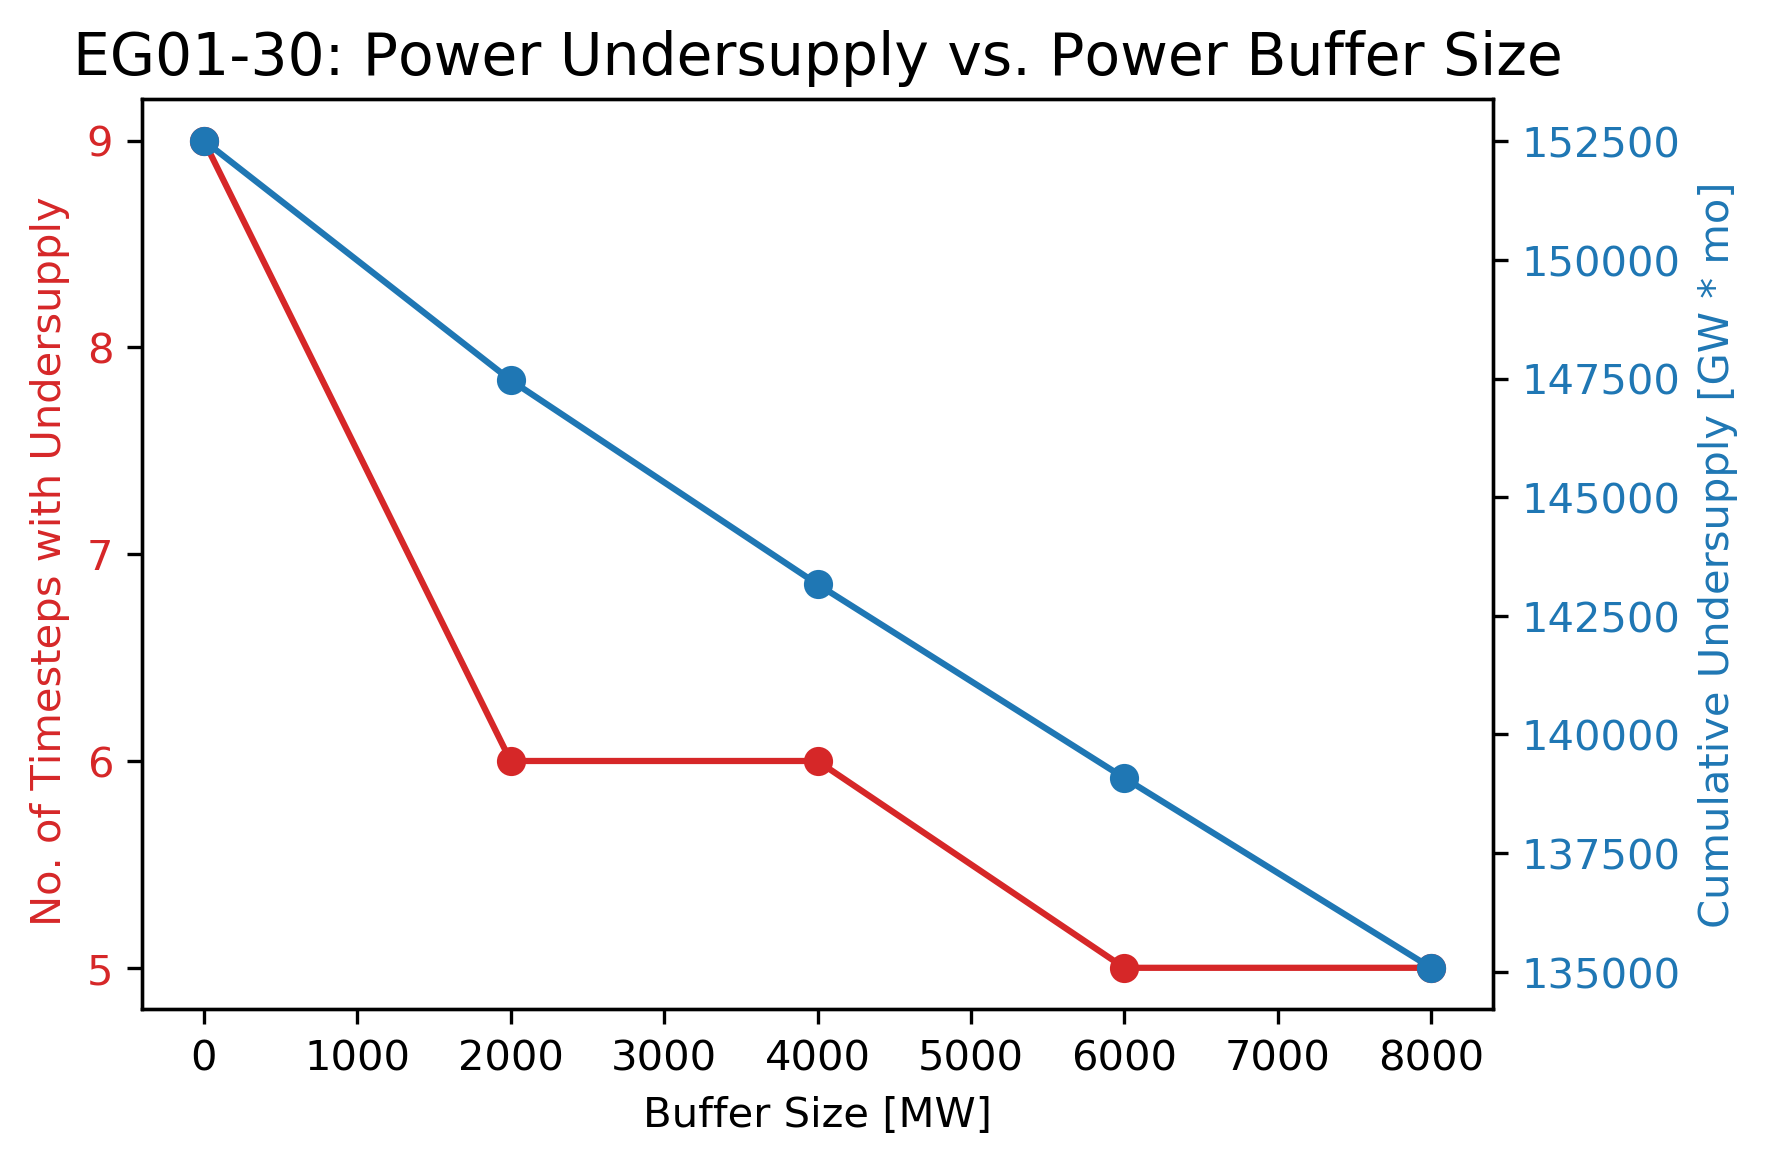
\includegraphics[width=\linewidth]{30-sens-buffer.png} 
		\caption{EG01-30: Power buffer size vs. cumulative undersupply}
		\label{fig:eg30-bufplot}
	\end{subfigure}
	\begin{subfigure}[t]{\textwidth}
		\centering
		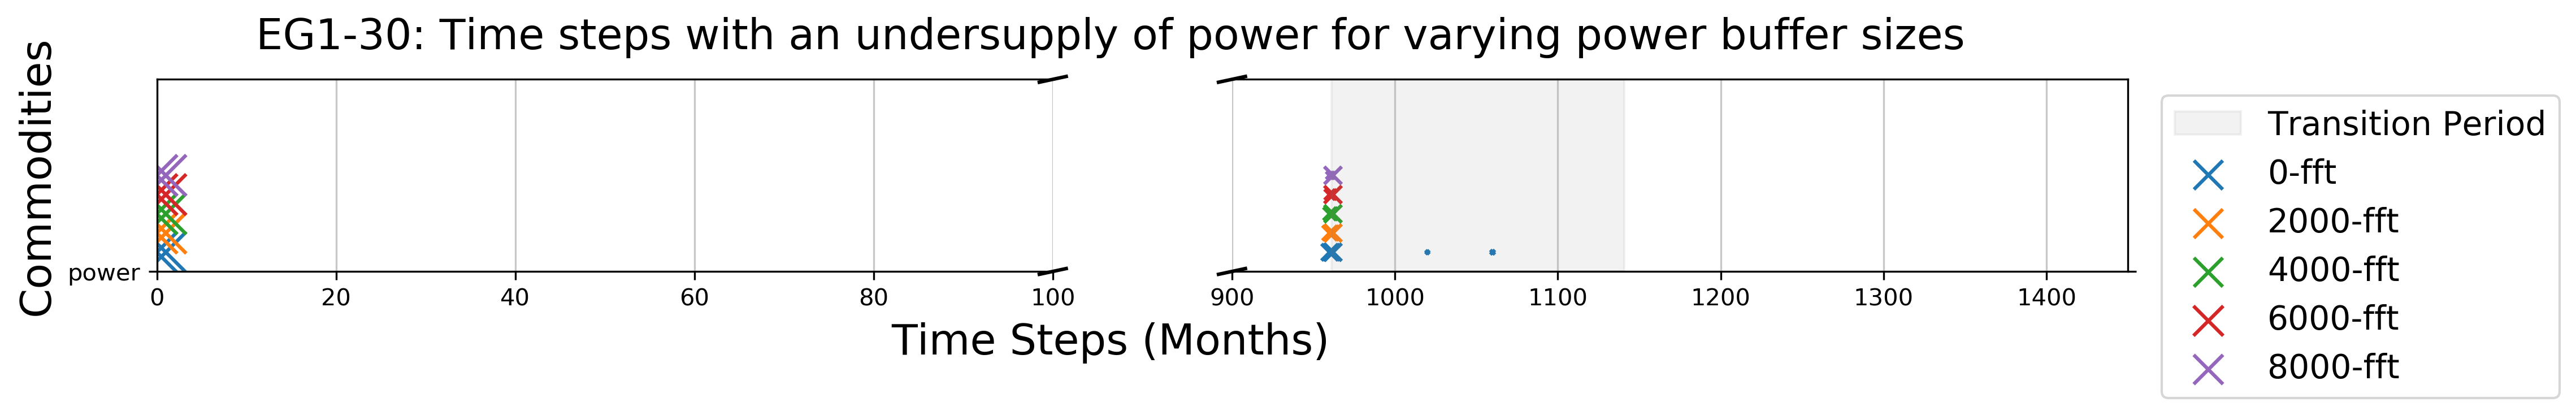
\includegraphics[width=\linewidth]{eg30-sa.png} 
		\caption{EG01-30: Time-dependent undersupply of power for varying power buffer sizes}
		\label{fig:eg30-dotplot}
	\end{subfigure}
	\hfill
	\caption{Sensitivity Analysis of Power buffer size on cumulative 
	undersupply of Power for the EG01-EG30 transition scenario 
	with linearly increasing power demand using the \texttt{fft} prediction method.}
	\label{fig:sabuffer}
\end{figure}

\begin{table}[h]
	\centering
	\caption{Dependency of the undersupply of Power on the buffer size 
	for EG01-EG30 transition scenarios with linearly 
	increasing power demand using the fft prediction method.}
	\label{tab:buff_size}
	\footnotesize
		\begin{tabular}{lll}
                \hline
                \textbf{Buffer [MW]}     & \textbf{Undersupply}               & \textbf{EG01-30} \\
		\hline
		0             & Time steps $[\#]$  & 9\\  
                      & Cumulative $[GW\cdot mo]$    & 152517 \\ \hline
        2000          & Undersupplied $[\#]$ & 6 \\  
        	      & Cumulative $[GW\cdot mo]$   & 147166 \\ \hline
        4000          & Time steps $[\#]$ & 6 \\  
				  & Cumulative $[GW\cdot mo]$     & 143166 \\ \hline
		6000          & Time steps $[\#]$  & 5 \\  
		& Cumulative $[GW\cdot mo]$     & 139083 \\ \hline
        8000          & Time steps $[\#]$  & 5  \\  
	              & Cumulative $[GW\cdot mo]$  & 135083 \\ \hline
	\end{tabular}
\end{table}

\subsection{Demonstration of Best Performance Model}
Table \ref{tab:bestinputs} 
shows \deploy input parameters for the 
EG01-EG30 transition scenario
that minimizes undersupply of power and minimizes 
the undersupply and under capacity of the other commodities
in the simulation. 
The need for commodity buffers is a reflection of reality
in which a supply buffer is usually maintained to ensure 
continuity in the event of an unexpected failure in the supply chain.

Figure \ref{fig:30stack} shows the
time-dependent deployment of reactor and supporting facilities 
for the EG01-30 linearly increasing power demand 
transition scenario.
\deploy automatically deploys reactor and supporting facilities 
to set up a supply chain to meet power demand
during a transition from \glspl{LWR} to \gls{MOX} \glspl{LWR} and 
\glspl{SFR} for EG01-30. 

\begin{table}[]
    \centering
    \caption{\deploy's input parameters for
	EG01-EG30 transition scenario
	that minimizes undersupply for power and minimizes 
	the undersupply and under capacity for other facilities. }
	\label{tab:bestinputs}
    \footnotesize
    \begin{tabular}{lll}
    \hline
                              & \textbf{\deploy Input Parameter}            & \textbf{EG01-30}            \\ \hline
    \multirow{4}{*}{\textbf{Required}} & Demand driving commodity   & Power              \\
                              & Demand equation {[}MW{]}   & 60000+250t/12        \\
                              & Prediction method          & fft                \\
                              & Deployment driving method  & Installed Capacity \\ \cline{1-3}
    \multirow{2}{*}{\textbf{Optional}} & Buffer type                & Absolute           \\
                              & Power buffer size {[}MW{]} & 8000               \\ 
                              & Transition Start Date [Month] & 960 (Year 80)\\ 
                              & Fleet share ratio [\%] & \gls{MOX} \gls{PWR}: 15\%, \gls{SFR}: 85\%\\ \hline
    \end{tabular}%
    \end{table}

    \begin{figure}[]
        \centering
        \begin{subfigure}[t]{\textwidth}
            \centering
            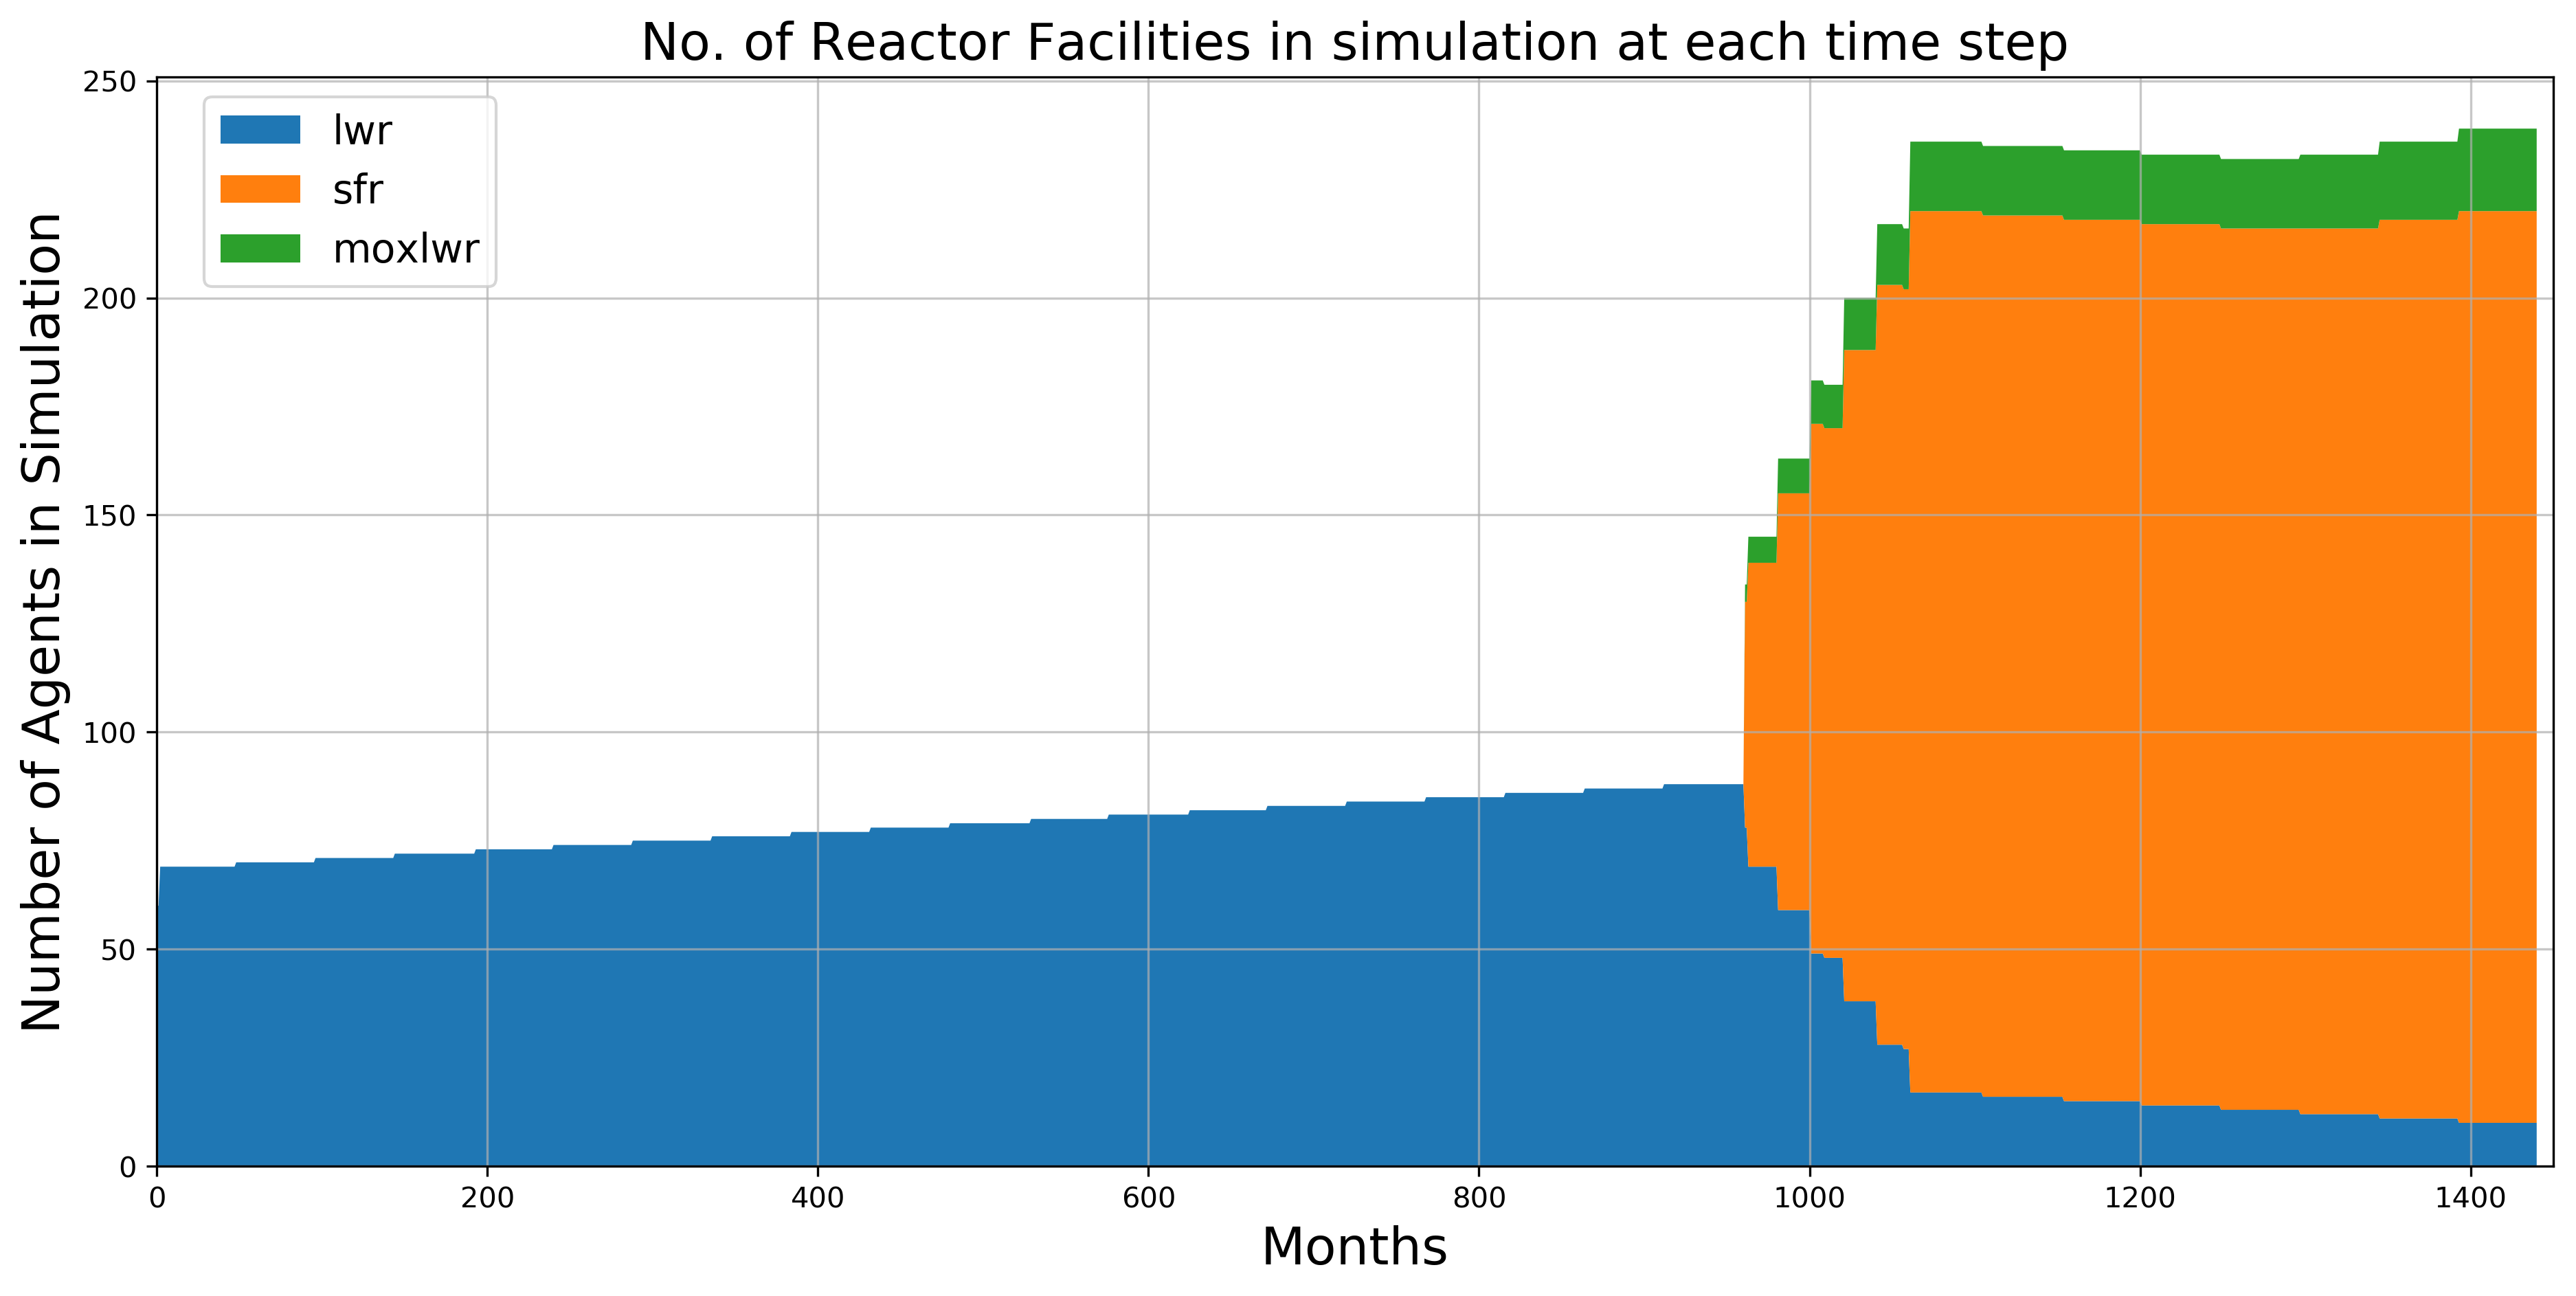
\includegraphics[width=\linewidth]{eg30-stack_reactor.png} 
            \caption{EG01-30: Reactor Deployment}
            \label{fig:30reactor}
        \end{subfigure}
        \vspace{1cm}
        \begin{subfigure}[t]{\textwidth}
            \centering
            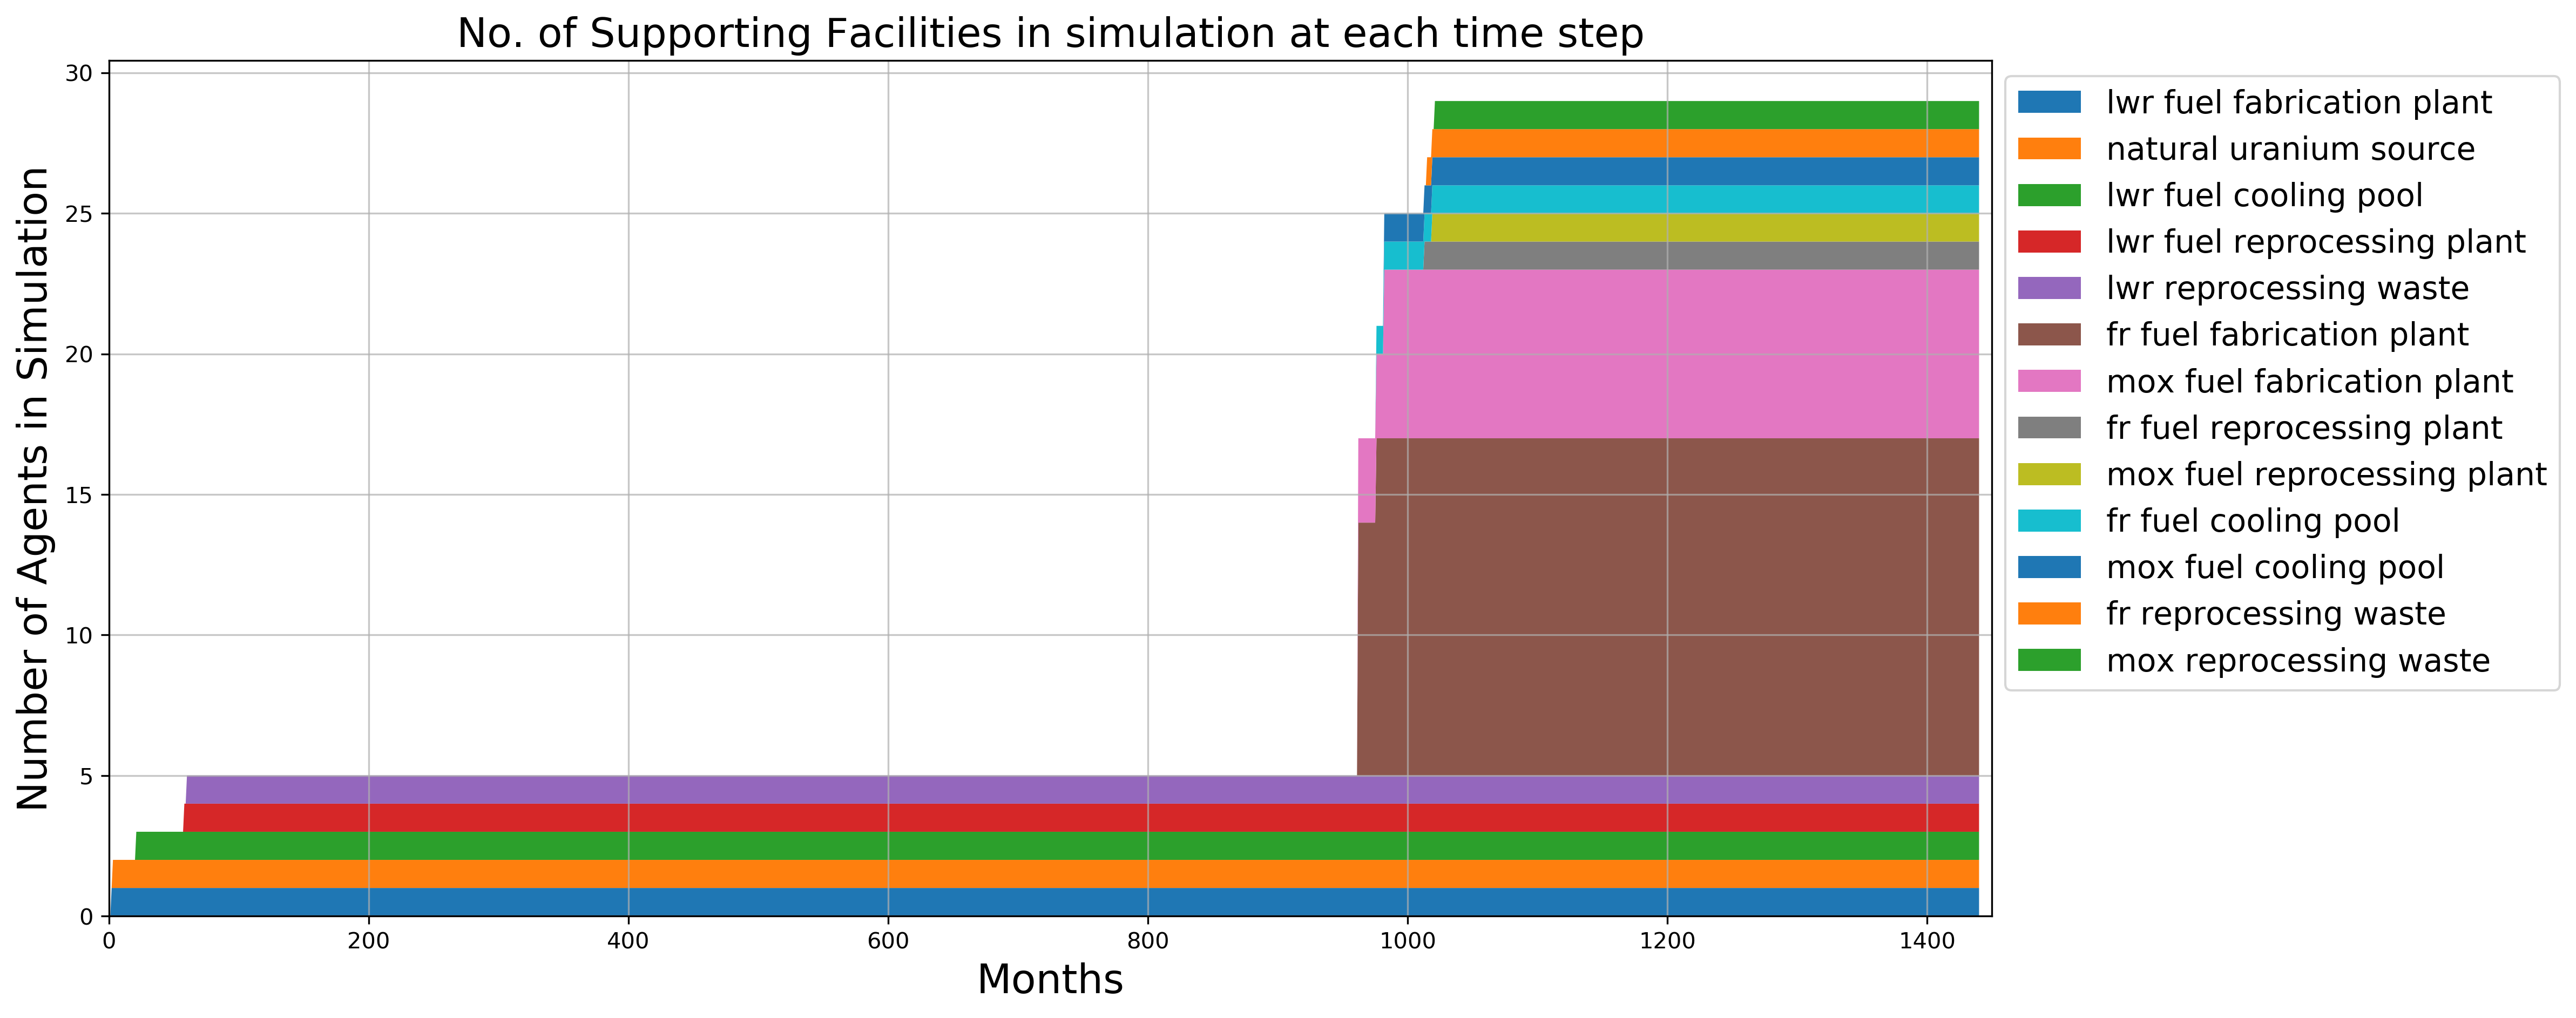
\includegraphics[width=\linewidth]{eg30-stack_support.png} 
            \caption{EG01-30: Supporting Facility Deployment}
            \label{fig:30support}
        \end{subfigure}
        \hfill
        \caption{Time dependent deployment of reactor and supporting facilities in 
        the EG01-30 linearly increasing power demand transition scenario. 
        \deploy automatically deploys reactor and supporting facilities 
        to setup a supply chain to meet linearly increasing power demand of $60000 + 250t/12$ MW
        during a transition from \glspl{LWR} to MOX LWRs and \glspl{SFR}. }
        \label{fig:30stack}
    \end{figure}
